\date{}
\title{}
\date{}
\begin{document}
\begin{frame}
    \titlepage
\end{frame}

\begin{frame}{last time}
    \begin{itemize}
    \item bandwidth-delay product and window size
        \begin{itemize}
        \item filling link at window size $\sim$ bandwidth-delay product
        \item can exceed `raw' link capacity by filling queues
        \item \myemph<2>{correction on next slide}
        \end{itemize}
    \item TCP
        \begin{itemize}
        \item sequence number = byte number for first data byte
        \item ack number = byte number 1 past first
        \end{itemize}
    \item ethernet frame format
    \item software-defined network motivation
        \begin{itemize}
        \item control plane versus data plane
        \item vendor-neutral programmable switches
        \end{itemize}
    \end{itemize}
\end{frame}

\begin{frame}{quiz note}
    \begin{itemize}
    \item managed to get confused talking about wrong answers re: Q3
        \begin{itemize}
        \item made mistake re: not consistently counting what needs to happen with/without losses
        \end{itemize}
    \item quiz site now has explanation of correct answer
    \end{itemize}
\end{frame}

\begin{frame}{not really empty/full queues (1)}
    \begin{itemize}
    \item showed we achieved maximum throughput at window size 20 = 2 ms RTT times 10 pkt/ms
    \item matches ``filling network'' idea
    \vspace{.5cm}
    \item<2-> but throughput collapsed at window size 22 = 2.2 ms RTT times 10 pkt/ms
    \item<2-> but queue could hold 20 packets, which would be 4 ms round-trip-time
        \begin{itemize}
        \item window size 40
        \end{itemize}
    \item<2-> what was going on?
    \end{itemize}
\end{frame}

\begin{frame}{not really empty/full queues (2)}
    \begin{itemize}
    \item calculation assumption: evenly spaced sending
    \item but data was from ``bursty'' sending
    \item example: send full window at start of connection
    \vspace{.5cm}
    \item means that queue occupency sometimes higher, sometimes lower
    \vspace{.5cm}
    \item overloading queue in temporary burst would cause throughput collapse
        \begin{itemize}
        \item even though queue not usually filled
        \end{itemize}
    \item won't get \textit{average} round-trip time = maximum possible
    \end{itemize}
\end{frame}

\begin{frame}{assignment Q\&A}
\end{frame}

\subsection{control v dataplane}
\begin{frame}{software defined networking (SDN)}
    \begin{itemize}
    \item movement toward \textit{programmable} networks
    \vspace{.5cm}
    \item ``software-defined''
        \begin{itemize}
        \item rules about how network works defined in ``normal'' software
        \end{itemize}
    \end{itemize}
\end{frame}

\begin{frame}{control plane and data plane}
    \begin{itemize}
    \item control plane
        \begin{itemize}
        \item decides \textit{how} to handle traffic
        \item ``slow path'', where complicated decisions are
        \end{itemize}
    \item data plane
        \begin{itemize}
        \item actually implements the decisions made by the control plane
        \item ``fast path'', implementing simple rules
        \end{itemize}
    \vspace{.5cm}
    \item probably what switches did internally before SDN was a thing
    \end{itemize}
\end{frame}

\begin{frame}{separate control/data plane}
    \begin{itemize}
    \item one SDN key idea: separate control and data plane
    \item allow new \myemph<2>{vendor-neutral} implementations of control plane
        \begin{itemize}
        \item requires standard interface for programming data plane
        \item most prominent example: OpenFlow
        \end{itemize}
    \item easily allows for central `control plane' server
        \begin{itemize}
        \item instead of separate control plane running on each switch/router
        \end{itemize}
    \end{itemize}
\end{frame}


\subsection{what is P4}

\begin{frame}{P4}
    \begin{itemize}
    \item P4 --- programming langauge for data planes
    \item intended to be compiled to run on fast switches
    \item includes `runtime' defining how control plane configures data plane
    \end{itemize}
\end{frame}

\begin{frame}{future P4 assignment}
    \begin{itemize}
    \item given: 
        \begin{itemize}
        \item simple P4 switch that doesn't know where to direct frames
        \item simpler controller (in Python) that configures switch
        \item simulated 4-machine network in VM
        \end{itemize}
    \item your task will be:
        \begin{itemize}
        \item have controller write static configuration to direct to right place
        \item modify data plane to send information to control plane
        \item have controller change configuration based on info from data plane
        \end{itemize}
    \item (we'll discuss more details later)
    \end{itemize}
\end{frame}


\subsection{P4 dataplane}
\subsubsection{switch parts}
\usetikzlibrary{arrows.meta,decorations.pathreplacing}
\begin{frame}[fragile,label=p4arch]{P4 switch architecture}
\begin{tikzpicture}
\tikzset{
    queue/.style={alt=<2>{fill=red!10,draw=red,ultra thick}},
    explain box/.style={
        align=left,at={(explain box top)},anchor=north,draw=red,very thick
    },
}
\begin{scope}[x=.7cm]
\foreach \x in {1,2,3,4} {
    \node[anchor=east] at (0, \x-.5) {IN$\rightarrow$};
    \node[anchor=west] at (17.5, \x-.5) {$\rightarrow$OUT};
    \foreach \noff in {0,8,16} {
        \begin{scope}[shift={(\noff, 0)},yshift=\x cm-1cm,y=0.9cm]
            \draw[queue,thick] (0, 0) rectangle (1.5, 1);
            \foreach \off in {.5,.7,.9,1.1,1.3} {
                \draw[queue,thick] (\off, 0) -- (\off, 1);
            }
        \end{scope}
    }
}
\coordinate (explain box top) at (8.5, -.7);
\tikzset{
    box/.style={draw,thick},
    box label/.style={font=\fontsize{9}{10}\selectfont},
    parserBox/.style={alt=<6>{fill=red!10}},
    deparserBox/.style={alt=<7>{fill=red!10}},
    ingressBox/.style={alt=<8>{fill=red!10}},
    egressBox/.style={alt=<8>{fill=red!10}},
};
\foreach \x/\name in {2/parser,4/ingress,6/deparser} {
    \draw[box,\name Box] (\x, 0) coordinate (\name-in-base) rectangle ++(1.6, 4) coordinate (\name-in-other-base) node[midway,box label,alias=x] (\name-in-label) {\name};
    \coordinate (\name-in-bottom-right) at (\name-in-base);
    \coordinate (\name-in-bottom-left) at (\name-in-base -| \name-in-other-base);
    \draw[box] (\x + 1.4, -.1) |- (\x - .2, .8-1) |- (\x-.1, 3.8); 
    \draw[box] (\x + 1.5, 0) |- (\x - .1, .9-1) |- (\x, 3.9); 
}
\foreach \x/\name in {10/parser,12/egress,14/deparser} {
    \draw[box,\name Box] (\x, 0) coordinate (\name-out-base) rectangle ++(1.6, 4) coordinate (\name-out-other-base) node[midway,box label] (\name-out label) {\name};
    \coordinate (\name-out-bottom-right) at (\name-out-base);
    \coordinate (\name-out-bottom-left) at (\name-out-base -| \name-out-other-base);
    \draw[box] (\x + 1.4, -.1) |- (\x - .2, .8-1) |- (\x-.1, 3.8); 
    \draw[box] (\x + 1.5, 0) |- (\x - .1, .9-1) |- (\x, 3.9); 
}
\end{scope}
\begin{visibleenv}<2>
    \node[explain box] {
        queues of frames to be processed \\
        if needed, hold packets in between processing steps 
    };
\end{visibleenv}
\begin{visibleenv}<3>
    \foreach \x in {in,out} {
        \draw[line width=.5mm,red,decorate,decoration={brace,mirror,raise=3mm,amplitude=2mm}]
            ([xshift=-.2cm]parser-\x-bottom-right) --
            ([xshift=.2cm]deparser-\x-bottom-left);
    }
    \node[explain box] {
        \textit{ingress} and \textit{egress} pipelines
    };
\end{visibleenv}
\begin{visibleenv}<4>
    \foreach \x in {in} {
        \draw[line width=.5mm,red,decorate,decoration={brace,mirror,raise=3mm,amplitude=2mm}]
            ([xshift=-.2cm]parser-\x-bottom-right) --
            ([xshift=.2cm]deparser-\x-bottom-left);
    }
    \node[explain box] {
        ingress pipeline: processes every input frame \\
        primary job: decide where to forward frame (if anywhere) 
    };
\end{visibleenv}
\begin{visibleenv}<5>
    \foreach \x in {out} {
        \draw[line width=.5mm,red,decorate,decoration={brace,mirror,raise=3mm,amplitude=2mm}]
            ([xshift=-.2cm]parser-\x-bottom-right) --
            ([xshift=.2cm]deparser-\x-bottom-left);
    }
    \node[explain box] {
        egress pipeline: process every output frame \\
        run one time for \myemph{each copy} output
    };
\end{visibleenv}
\begin{visibleenv}<6>
    \foreach \x in {in,out} {
        \draw[line width=.5mm,red,decorate,decoration={brace,mirror,raise=3mm,amplitude=2mm}]
            ([xshift=-.2cm]parser-\x-bottom-right) --
            ([xshift=.2cm]parser-\x-bottom-left);
    }
    \node[explain box] {
        parser: decode frame fields into temporary storage
    };
\end{visibleenv}
\begin{visibleenv}<7>
    \foreach \x in {in,out} {
        \draw[line width=.5mm,red,decorate,decoration={brace,mirror,raise=3mm,amplitude=2mm}]
            ([xshift=-.2cm]deparser-\x-bottom-right) --
            ([xshift=.2cm]deparser-\x-bottom-left);
    }
    \node[explain box] {
        deparser: converted decoded fields back into bytes for network
    };
\end{visibleenv}
\begin{visibleenv}<8>
    \foreach \x in {ingress-in,egress-out} {
        \draw[line width=.5mm,red,decorate,decoration={brace,mirror,raise=3mm,amplitude=2mm}]
            ([xshift=-.2cm]\x-bottom-right) --
            ([xshift=.2cm]\x-bottom-left);
    }
    \node[explain box] {
        ``match/action pipelines'' \\
        do series of table lookups based on parsed fields \\
        each table lookup specifies next action
    };
\end{visibleenv}
\end{tikzpicture}
\end{frame}

\begin{frame}[fragile]{P4: switch parts}
\begin{Verbatim}
V1Switch(
MyParser(),
MyVerifyChecksum(),
MyIngress(),
MyEgress(),
MyComputeChecksum(),
MyDeparser()
) main;
\end{Verbatim}
\begin{itemize}
\item code to declare instance of dataplane from functions for each part
\item will look at most of these components
    \begin{itemize}
    \item won't have reason to change verify/compute checksum
    \end{itemize}
\end{itemize}
\end{frame}

\subsubsection{header management}
\usetikzlibrary{arrows.meta,decorations.pathreplacing}


\begin{frame}[fragile]{P4: declaring headers (1)}
\providecommand{\vemphA}[1]{\myemph<2>{#1}}
\providecommand{\vemphB}[1]{\myemph<3>{#1}}
\providecommand{\vemphC}[1]{\myemph<4>{#1}}
\providecommand{\vemphD}[1]{\myemph<5>{#1}}
\begin{Verbatim}[fontsize=\small,commandchars=\\@~]
typedef bit<48> macAddr_t;
\vemphA@@header~ ethernet_t~ {
    macAddr_t srcAddr;
    macAddr_T dstAddr;
    bit<16>   etherType;
}
\end{Verbatim}
\begin{itemize}
\item<2-> kinda like \Verb|typedef struct { ... } ethernet_t;|
\item<3-> order needs to \textit{exactly} match what's sent on network
    \begin{itemize}
    \item switch will do bit-by-bit copy into this struct
    \end{itemize}
\end{itemize}
\end{frame}

\begin{frame}[fragile]{P4: declaring headers (2)}
\providecommand{\vemphA}[1]{\myemph<2>{#1}}
\providecommand{\vemphB}[1]{\myemph<3>{#1}}
\providecommand{\vemphC}[1]{\myemph<4>{#1}}
\providecommand{\vemphD}[1]{\myemph<5>{#1}}
\begin{Verbatim}[fontsize=\small,commandchars=\\@~]
\vemphA@struct headers~ {
    \vemphB@ethernet_t~   ethernet;
    \vemphB@ipv4_t~       ipv4;
    \vemphB@ipv6_t~       ipv6;
}
\end{Verbatim}
\begin{itemize}
\item<2-> struct of all possible headers
    \begin{itemize}
    \item from all layers the switch/router handles
    \item not all frames will use all of them, some may be mutually exclusive
    \item order does not need to match frame storage (will write code to handle that)
    \end{itemize}
\item<3-> references header types defined previously
\end{itemize}
\end{frame}

% FIXME: hilite parts with explanation
\begin{frame}[fragile]{P4: parsing}
\begin{Verbatim}
parser MyParser(
    packet_in packet,
    out headers hdr,
    inout metadata meta,
    inout standard_metadata_t standard_metadata) {
\end{Verbatim}
\begin{itemize}
\item function modifies `out' parameters instead of returning
\item parser function --- takes parameters:
    \begin{itemize}
    \item packet --- the input frame
    \item headers --- extracted headers (\texttt{struct headers})
    \item meta --- program's local variables about frame (\texttt{struct metadata})
    \item standard\_metadata --- info for system about frame
        \begin{itemize}
        \item where frame came from, where it should go, etc.
        \end{itemize}
    \end{itemize}
\end{itemize}
\end{frame}

\begin{frame}[fragile]{P4: parsing}
\providecommand{\vemphA}[1]{\myemph<2>{#1}}
\providecommand{\vemphB}[1]{\myemph<3>{#1}}
\providecommand{\vemphC}[1]{\myemph<4>{#1}}
\providecommand{\vemphD}[1]{\myemph<5>{#1}}
\begin{Verbatim}[fontsize=\small,commandchars=\\@~]
parser MyParser(...) {
    \vemphA@state~ start {
        \vemphB@transition~ \vemphC@parse_ethernet~;
    }
    \vemphA@state~ \vemphC@parse_ethernet~ {
        \vemphD@packet.extract(hdr.ethernet);~
        \vemphB@transition~ select(hdr.ethernet.etherType) {
            TYPE_IPV4: parse_ipv4;
            TYPE_IPV6: parse_ipv6
            default: accept;
        }
    }
    ....
}
\end{Verbatim}
\begin{tikzpicture}[overlay,remember picture]
    \begin{visibleenv}<2>
    \node[align=left,draw=red,fill=white,very thick] at (current page.center) {
        functions written as state machine \\
        exectuion starts in state \texttt{start} \\
        follows instructions in each state
    };
    \end{visibleenv}
    \begin{visibleenv}<3-4>
    \node[align=left,draw=red,fill=white,very thick] at ([yshift=-1cm]current page.center) {
        transition statements say which state to go to next  \\
        can be conditional using switch-statement-like syntax
    };
    \end{visibleenv}
    \begin{visibleenv}<5>
    \node[align=left,draw=red,fill=white,very thick] at ([yshift=-1.5cm]current page.center) {
        \texttt{extract} operation copies from packet \\
        into specific \texttt{header} object
    };
    \end{visibleenv}
\end{tikzpicture}
\end{frame}

\subsubsection{exercise}
\begin{frame}{exercise: header representation (1)}
    \begin{itemize}
    \item let's say packet format is:
        \begin{itemize}
        \item 16 bit source address
        \item 16 bit destination address
        \item 1 bit flag ``is timestamp present''
        \item 1 bit flag ``is data present'
        \item 6 bits unused
        \item (optional) 32-bit timestamp
        \item (optional) 16-bit data size
        \item (optional) data
        \end{itemize}
    \item how to represent this?
        \begin{itemize}
        \item how many structs?
        \item what's in the \texttt{header \{\ldots\}}?
        \end{itemize}
    \end{itemize}
\end{frame}

\begin{frame}{}
\end{frame}

\begin{frame}[fragile]{exercise: header parsing}
\begin{Verbatim}[fontsize=\small]
struct basic_hdr_t {
    bit<16> src; bit<16> dst;
    bit<1> has_timestamp; bit<1> has_data; bit<6> unused;
};
struct timestamp_t {
    bit<32> timestamp;
}
struct data_hdr_t {
    bit<16> size;
}
\end{Verbatim}
\begin{itemize}
\item what states/transitions in parser?
\end{itemize}
\end{frame}

\begin{frame}[fragile]{states/transitions}
\begin{itemize}
\item parse\_basic:
    \begin{itemize}
    \item has\_timestamp: to parse\_timestamp:
    \item has\_data: to parse\_data
    \item otherwise: accept
    \end{itemize}
\item parse\_timestamp:
    \begin{itemize}
    \item has\_data: to parse\_data:
    \item otherwise: accept
    \end{itemize}
\item parse\_data: then accept
\end{itemize}
\end{frame}

\subsubsection{ingress processing}
\usetikzlibrary{arrows.meta,decorations.pathreplacing}


\begin{frame}[fragile]{P4: ingress processing}
\providecommand{\vemphA}[1]{\myemph<2>{#1}}
\providecommand{\vemphB}[1]{\myemph<3>{#1}}
\providecommand{\vemphC}[1]{\myemph<4>{#1}}
\providecommand{\vemphD}[1]{\myemph<5>{#1}}
\begin{itemize}
\item example: send \textit{everything} to output port number 4
\end{itemize}
\begin{Verbatim}[fontsize=\small,commandchars=\\@~]
control MyIngress(...) {
    apply {
        \vemphA@standard_metadata.egress_spec = 4;~
    }
}
\end{Verbatim}
\begin{tikzpicture}[overlay,remember picture]
    \begin{visibleenv}<2>
    \node[align=left,draw=red,fill=white,ultra thick] at ([yshift=-2cm]current page.center) {
        standard\_metadata --- `hard-coded' phase reads \texttt{egress\_spec} \\
        ~ \\
        special \texttt{egress\_spec} value for ``discard frame''
    };
    \end{visibleenv}
\end{tikzpicture}
\end{frame}

\begin{frame}{switch decisions}
    \begin{itemize}
    \item most decisions switches/routers make are table lookups
    \vspace{.5cm}
    \item take field from packet (e.g. destination)
    \item lookup in table what to do with that
        (e.g. send to port X, throw error, etc.)
    \vspace{.5cm}
    \item P4 has special syntax for tables and table lookups
    \end{itemize}
\end{frame}

\begin{frame}[fragile]{P4: tables}
\providecommand{\vemphA}[1]{\myemph<2>{#1}}
\providecommand{\vemphB}[1]{\myemph<3>{#1}}
\providecommand{\vemphC}[1]{\myemph<4>{#1}}
\providecommand{\vemphD}[1]{\myemph<5>{#1}}
\begin{Verbatim}[fontsize=\small,commandchars=\\@~]
\vemphA@table~ mac_dst_exact {
    \vemphB@key~ = {
        \vemphB@hdr.ethernet.dstAddr~ : \vemphC@exact~;
    }
    \vemphB@actions~ = {
        drop,
        forward_to,
    }
    size = 1024;
    default_action = drop();
}
\end{Verbatim}
\begin{tikzpicture}[overlay,remember picture]
\tikzset{
    box/.style={
        align=left,
        draw=red,
        fill=white,
        ultra thick,
        anchor=west,
        at={([xshift=1cm]current page.center)},
    },
}
    \begin{visibleenv}<2>
    \node[box] {
        declare a table with a name \\
        done has part of ingress/outgress
    };
    \end{visibleenv}
    \begin{visibleenv}<3>
    \node[box] {
        key/value structure \\
        keys usually from headers \\
        values are actions to run
    };
    \end{visibleenv}
    \begin{visibleenv}<4>
    \node[box] {
        here, each table entry \\
        contains whole address \\
        P4 also supports \\
        partially matched keys
    };
    \end{visibleenv}
\end{tikzpicture}
\end{frame}

\begin{frame}{P4 table key types}
    \begin{itemize}
    \item exact --- full entry
    \item lpm --- longest prefix match
        \begin{itemize}
        \item table entries contain `prefixes' of header field(s)
        \item we'll see motivation for this when we talk about routing
        \item if multiple entries match, take longest one
        \end{itemize}
    \item ternary --- 0/1/don't care
        \begin{itemize}
        \item table entries contain key and mask
        \item entry matches if bits included in mask match
        \item other view: keys represented with 0/1/don't care `trits'
        \end{itemize}
    \end{itemize}
\end{frame}

\begin{frame}{content-addressable memory}
    \begin{itemize}
    \item high-end routers/switches have \textit{content addressable memory} (CAM)
    \item \ldots including \textit{ternary content addressable memory} (TCAM)
    \vspace{.5cm}
    \item = hardware that implements a table lookup
        \begin{itemize}
        \item `content' $\approx$ key being looked up
        \item looks kinda like highly associative cache
        \item probably lots of comparators
        \end{itemize}
    \item allows multigigabit frame processing speeds
    \item P4 goal: P4 programs compile to use CAM/TCAM when available
    \end{itemize}
\end{frame}

\begin{frame}{aside: TCAM cost}
    \begin{itemize}
    \item 2.7x more transistors than SRAM (common cache technology)
    \item probably much more power than SRAM
    \item hard to find recent quotes for price/power
    \item but probably 10s of dollars per megabyte
        \begin{itemize}
        \item e.g., secondary market price of Broadcom chip with 40Mbit of this is $\sim$\$180
        \item chip needs 80W heatsink, max 900MHz clock rate
        \item but chip has a bunch of other functionality, of course
        \end{itemize}
    \end{itemize}
\end{frame}

\begin{frame}[fragile]{P4: using a table}
\providecommand{\vemphA}[1]{\myemph<2>{#1}}
\providecommand{\vemphB}[1]{\myemph<3>{#1}}
\providecommand{\vemphC}[1]{\myemph<4>{#1}}
\providecommand{\vemphD}[1]{\myemph<5>{#1}}
\begin{Verbatim}[fontsize=\small,commandchars=\\@~]
control MyIngress(...) {
    ...
    table mac_dst_exact = { 
        /* seen earlier */ ...
    }
    apply {
        \vemphA@mac_dst_exact.apply();~
    }
}
\end{Verbatim}
\begin{tikzpicture}[overlay,remember picture]
\tikzset{
    box/.style={
        align=left,
        draw=red,
        fill=white,
        ultra thick,
        anchor=west,
        at={([xshift=1cm]current page.center)},
    },
}
    \begin{visibleenv}<2>
    \node[box] {
        apply operation invokes the action specified by the table
    };
    \end{visibleenv}
\end{tikzpicture}
\end{frame}

\begin{frame}[fragile]{P4: actions}
\providecommand{\vemphA}[1]{\myemph<2>{#1}}
\providecommand{\vemphB}[1]{\myemph<3>{#1}}
\providecommand{\vemphC}[1]{\myemph<4>{#1}}
\providecommand{\vemphD}[1]{\myemph<5>{#1}}
\begin{Verbatim}[fontsize=\small,commandchars=\\@~]
control MyIngress(...) {
    \vemphA@action drop()~ {
        mark_to_drop(\vemphB@standard_metadata~);
    }
    \vemphA@action forward_to(egressSpec_t port)~ {
        \vemphB@standard_metadata.egress_spec = port;~
    }
    \vemphA@action mark_and_forward(egressSpec_t port)~ {
        \vemphC@hdr.some_proto.value~ = 1;
        \vemphB@standard_metadata.egress_spec = port;~
    }
    ...
}
\end{Verbatim}
\begin{tikzpicture}[overlay,remember picture]
\tikzset{
    box/.style={
        align=left,
        draw=red,
        fill=white,
        ultra thick,
        anchor=north,
        at={([yshift=-1cm]current page.center)},
    },
}
    \begin{visibleenv}<2>
    \node[box] {
        actions basically function calls for packet \\
        can include parameters that are stored in table
    };
    \end{visibleenv}
    \begin{visibleenv}<3>
    \node[box] {
        typically, actions set standard metadata \\
        to indicate where to send frame next \\
        ~ \\
        actual sending/not sending frame done later
    };
    \end{visibleenv}
    \begin{visibleenv}<4>
    \node[box] {
        actions can also edit packet headers \\
        or do other table lookups \\
        (which we will need in the future) 
    };
    \end{visibleenv}
\end{tikzpicture}
\end{frame}

\begin{frame}[fragile]{P4: special actions}
    \begin{itemize}
    \item some ways switch can direct packet (incomplete list)
    \vspace{.5cm}
    \item send to the control plane
        \begin{itemize}
        \item special output port that goes to `general purpose' CPU
        \end{itemize}
    \item multicast/broadcast to multiple ports
        \begin{itemize}
        \item control plane can set \textit{multicast groups}
        \item makes multiple copies of packets
        \end{itemize}
    \end{itemize}
\end{frame}


\subsubsection{exercise}
\begin{frame}{exercise}
    \begin{itemize}
    \item suppose we want to implement the following policy:
        \begin{itemize}
        \item by default, packets sent to servers A, B, C, and D are dropped
        \item specific machines are given permission to contact server A
        \item the same is true for servers B and C and D
        \item some specific machines are give access to contact all servers
        \end{itemize}
    \item what tables would be useful to have?
        \begin{itemize}
        \item what keys?
        \item what match strategy?
        \end{itemize}
    \end{itemize}
\end{frame}

\subsubsection{egress processing}
\begin{frame}{egress processing}
    \begin{itemize}
    \item same as ingress processing but different function
    \vspace{.5cm}
    \item usage in upcoming assignment:
        \begin{itemize}
        \item ingress step duplicates packet to all output ports
        \item egress step step runs on each duplicate, drops excess one
        \end{itemize}
    \end{itemize}
\end{frame}


\subsection{P4 controlplane}

\begin{frame}<1>[label=controlToC]{P4: control plane}
    \begin{itemize}
    \item P4 control plane is a program
    \vspace{.5cm}
    \item sends commands to one or more switches:
        \begin{itemize}
        \item \myemph<2>{load P4 program into data plane}
        \item \myemph<3>{set table entries}
        \item \myemph<4>{configure multicast groups}
        \item \myemph<5>{receive frames to process them}
        \end{itemize}
    \end{itemize}
\end{frame}

\begin{frame}{aside: wrappers}
    \begin{itemize}
    \item I'll show code from a P4 controller for upcoming assignment
    \item written in Python, using custom library to make things convenient
    \item works with softawre based reference switch
    \vspace{.5cm}
    \item no requirement to use Python or other specific language
        \begin{itemize}
        \item controller sends commands over network/IPC to data plane
        \end{itemize}
    \item real raw code has more boilerplate/etc.
    \item probably several things different for hardware-based switches
    \end{itemize}
\end{frame}

\againframe<2>{controlToC}

\begin{frame}[fragile]{P4: loading P4 program}
\providecommand{\vemphA}[1]{\myemph<2>{#1}}
\providecommand{\vemphB}[1]{\myemph<3>{#1}}
\providecommand{\vemphC}[1]{\myemph<4>{#1}}
\providecommand{\vemphD}[1]{\myemph<5>{#1}}
\begin{Verbatim}[fontsize=\small,commandchars=\\@~]
p4info_helper =  ....
switch = ....
\vemphA@switch.MasterArbitrationUpdate()~
switch.\vemphB@SetForwardingPipelineConfig~(
    p4info=p4info_helper.p4info,
    \vemphC@bmv2_json_file_path=bmv2_file_path~
)
\end{Verbatim}
\begin{tikzpicture}[overlay,remember picture]
\tikzset{
    box/.style={
        align=left,
        draw=red,
        fill=white,
        ultra thick,
        anchor=north,
        at={([yshift=-1cm]current page.center)},
    },
}
    \begin{visibleenv}<2>
    \node[box] {
        swtich supports having primary + backup controller, \\
        so need to indicate this is primary controller now \\
    };
    \end{visibleenv}
    \begin{visibleenv}<3>
    \node[box] {
        ``forwarding pipeline'' = dataplane
    };
    \end{visibleenv}
    \begin{visibleenv}<4>
    \node[box] {
        P4 code compiled to file to load, specified here
    };
    \end{visibleenv}
\end{tikzpicture}
\end{frame}

\againframe<3>{controlToC}

\begin{frame}[fragile]{P4: setting table entries}
\providecommand{\vemphA}[1]{\myemph<2>{#1}}
\providecommand{\vemphB}[1]{\myemph<3>{#1}}
\providecommand{\vemphC}[1]{\myemph<4>{#1}}
\providecommand{\vemphD}[1]{\myemph<5>{#1}}
\begin{Verbatim}[fontsize=\small,commandchars=\\@~]
\vemphD@write_or_overwrite_table_entry~(
    \vemphA@p4info_helper=p4info_helper, switch=switch,~
    table_name='\vemphB@MyIngress.mac_dst_exact~',
    match_fields={
        'hdr.ethernet.dstAddr': \vemphC@some_address~,
    },
    action_name='forward_to',
    action_params={'port': port},
)
\end{Verbatim}
\begin{tikzpicture}[overlay,remember picture]
\tikzset{
    box/.style={
        align=left,
        draw=red,
        fill=white,
        ultra thick,
        anchor=north,
        at={([yshift=-1cm]current page.center)},
    },
}
    \begin{visibleenv}<2>
    \node[box] {
        p4info\_helper, switch objects created by setup code
    };
    \end{visibleenv}
    \begin{visibleenv}<3>
    \node[box] {
        full name of table, including stage it is defined in
    };
    \end{visibleenv}
    \begin{visibleenv}<4>
    \node[box] {
        match value --- format would be different \\
        if key was \texttt{lpm} or \texttt{ternary} \\
        instead of exact match
    };
    \end{visibleenv}
    \begin{visibleenv}<5>
    \node[box] {
        \texttt{write\_or\_overwrite\_table\_entry} not the `raw' function \\
        (one I wrote based on one P4 tutorial authors wrote) \\
        uses gRPC (remote procedure call) library, which adds some extra steps
    };
    \end{visibleenv}
\end{tikzpicture}
\end{frame}

\againframe<4>{controlToC}
\begin{frame}[fragile]{P4: multicast groups}
\providecommand{\vemphA}[1]{\myemph<2>{#1}}
\providecommand{\vemphB}[1]{\myemph<3>{#1}}
\providecommand{\vemphC}[1]{\myemph<4>{#1}}
\providecommand{\vemphD}[1]{\myemph<5>{#1}}
\begin{Verbatim}[fontsize=\small,commandchars=\\@~]
switch.Write\vemphC@PRE~Entry(
    p4info_helper.buildMulticastGroupEntry(
        \vemphA@multicast_group_id=1~, 
        \vemphB@replicas~=[
            {'egress_port': 1, 'instance': 0},
            {'egress_port': 2, 'instance': 0},
            {'egress_port': 3, 'instance': 0},
            {'egress_port': 4, 'instance': 0},
        ]
    )
)
\end{Verbatim}
\begin{tikzpicture}[overlay,remember picture]
\tikzset{
    box/.style={
        align=left,
        draw=red,
        fill=white,
        ultra thick,
        anchor=north,
        at={([yshift=-1cm]current page.center)},
    },
}
    \begin{visibleenv}<2>
    \node[box] {
        in P4 dataplane code can write \\
        \texttt{standard\_metadata.mcast\_grp = 1} to use this
    };
    \end{visibleenv}
    \begin{visibleenv}<3>
    \node[box] {
        list of ports to output to when group selected \\
        ~ \\
        \texttt{instance} can be inspected by dataplane code \\
        for the egress step
    };
    \end{visibleenv}
    \begin{visibleenv}<4>
    \node[box] {
        PRE = packet replication engine \\
        ~ \\
        supports multicast groups (shown) and ``clone sessions'' (not shown) \\
        (clone sessions make extra copy of packet, \\
        but process original normally)
    };
    \end{visibleenv}
\end{tikzpicture}
\end{frame}

\againframe<5>{controlToC}
\begin{frame}[fragile]{P4: receiving frame}
\providecommand{\vemphA}[1]{\myemph<2>{#1}}
\providecommand{\vemphB}[1]{\myemph<3>{#1}}
\providecommand{\vemphC}[1]{\myemph<4>{#1}}
\providecommand{\vemphD}[1]{\myemph<5>{#1}}
\begin{Verbatim}[fontsize=\small,commandchars=\\@~]
    for item in switch.stream_msg_resp:
        if item.HasField('packet'):
            do_something_with(\vemphA@item.packet.payload~,
                              \vemphB@item.packet.metadata~)
\end{Verbatim}
\begin{tikzpicture}[overlay,remember picture]
\tikzset{
    box/.style={
        align=left,
        draw=red,
        fill=white,
        ultra thick,
        anchor=north,
        at={([yshift=0cm]current page.center)},
    },
}
    \begin{visibleenv}<2>
    \node[box] {
        payload = bytes of frame  \\
        (what would normally be sent on network)
    };
    \end{visibleenv}
    \begin{visibleenv}<3>
    \node[box] {
        extra metadata can be set by dataplane \\
        example: which port packet came from
    };
    \end{visibleenv}
\end{tikzpicture}
\end{frame}


\section{basic Ethernet switching / MAC learning}

%\againframe<10>{ethernetFormat}

% FIXME: show before/after wireshark picture form assignment

\usetikzlibrary{arrows.meta,calc,matrix,shapes}
\providecommand{\computer}{%
    
\includegraphics[width=1cm]{../common/Noun_project_216.pdf}
}
\providecommand{\switch}{%
    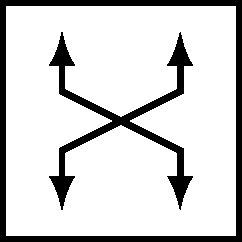
\includegraphics[width=0.9cm]{../common/fig-switch.pdf}
}
\providecommand{\router}{%
    
\includegraphics[width=0.9cm]{../common/fig-router.pdf}
}

\begin{frame}{network and switch tables}
\begin{tikzpicture}
\tikzset{
    computer/.style={inner sep=0mm,outer sep=0mm,execute at begin node={\computer}},
    switch/.style={inner sep=0mm,outer sep=0mm,execute at begin node={\switch}},
    connect/.style={draw,very thick,Latex-Latex},
    connect big/.style={draw,ultra thick,Latex-Latex},
    port/.style={pos=0.95,fill=white,circle,draw,inner sep=0mm},
    port beginning/.style={pos=0.05,fill=white,circle,draw,inner sep=0mm},
    mac label/.style={
        visible on=<2->,draw,fill=white,inner sep=1mm,font=\tiny\tt,
        alt=<2>{text=red,draw=red},
    },
    route table/.style={
        matrix of nodes,ampersand replacement=\&,
        column 1/.style={nodes={draw,thick,text width=2.5cm,font=\tiny\tt,text depth=0mm,minimum height=0.5cm,inner sep=1mm}},
        column 2/.style={nodes={draw,thick,text width=.5cm,font=\small\tt,text depth=0mm,minimum height=0.5cm,inner sep=1mm}},
        row 1/.style={nodes={draw=none,font=\small}},
    }
}
\foreach \x/\d/\mc/\dir in {15/8cm/AA/north,45/3cm/BB/north,90/2cm/CC/north,135/3cm/DD/north,180/4cm/EE/north,300/4cm/FF/south} {
    \node[computer,label={[mac label,]\dir:00:11:22:33:44:\small\mc}] (c-\x) at (\x:\d) {};
}
\node[switch,alt=<4>{fill=red!10}] (s1) at (4,-0.5) {};
\begin{visibleenv}<4->
\matrix[route table,alt=<4>{fill=red!10},anchor=north west] (s1 table) at ([xshift=1cm,yshift=.5cm]s1.north east) {
dst MAC addr \& port \\
00:11:22:33:44:\small AA \& 1 \\
00:11:22:33:44:\small BB \& 2 \\
00:11:22:33:44:\small CC \& 4 \\
00:11:22:33:44:\small DD \& 4 \\
00:11:22:33:44:\small EE \& 4 \\
00:11:22:33:44:\small FF \& 3 \\
};
\draw[dotted,thick] (s1.north east) -- (s1 table-2-1.north west);
\draw[dotted,thick] (s1.south east) -- (s1 table-7-1.south west);
\end{visibleenv}
\node[switch,alt=<3>{fill=red!10}] (s2) at (-1,0.5) {};
\begin{visibleenv}<3->
\matrix[route table,alt=<3>{fill=red!10},anchor=north east] (s2 table) at ([xshift=2cm]s2.south west) {
dst MAC addr \& port \\
00:11:22:33:44:\small AA \& 1 \\
00:11:22:33:44:\small BB \& 1 \\
00:11:22:33:44:\small CC \& 2 \\
00:11:22:33:44:\small DD \& 3 \\
00:11:22:33:44:\small EE \& 4 \\
00:11:22:33:44:\small FF \& 2 \\
};
\draw[dotted,thick] (s2.south east) -- (s2 table-2-2.north east);
\draw[dotted,thick] (s2.south west) -- (s2 table-2-1.north west);
\end{visibleenv}
\draw[connect] (c-15) -- (s1) node[port] {1};
\draw[connect] (c-45) -- (s1) node[port] {2};
\draw[connect] (c-300) -- (s1) node[port] {3};
\draw[connect] (c-90) -- (s2) node[port] {2};
\draw[connect] (c-135) -- (s2) node[port] {3};
\draw[connect] (c-180) -- (s2) node[port] {4};
\draw[connect big] (s1) -- (s2) node[port beginning] {4} node [port] {1};
\end{tikzpicture}
\end{frame}

\begin{frame}{constructing switch tables}
    \begin{itemize}
    \item could have system administrator input these by hand
        \begin{itemize}
        \item through an SSH-like interface, probably
        \end{itemize}
    \item works, but error-prone, hard to change, etc.
    \vspace{.5cm}
    \item<2-> alternative: switch should figure it out
    \end{itemize}
\end{frame}

\begin{frame}{MAC learning}
\begin{tikzpicture}
\tikzset{
    route table/.style={
        matrix of nodes,ampersand replacement=\&,
        column 1/.style={nodes={draw,thick,text width=2.5cm,font=\tiny\tt,text depth=1mm,text height=3.5mm,minimum height=0.6cm,inner sep=1mm}},
        column 2/.style={nodes={draw,thick,text width=1cm,font=\small\tt,text depth=1mm,text height=3.5mm,minimum height=0.6cm,inner sep=1mm}},
        row 1/.style={nodes={draw=none,font=\small}},
    }
}
\matrix[label={north:forwarding table},route table,draw,very thick,anchor=north east] (table) {
dst MAC addr \& port \\
|[alt={<5,7>{fill=red!10}}]| \alt<5->{00:11:22:33:44:AA}{~}
    \& |[alt={<5,7>{fill=red!10}}]| \alt<5->{2}{~} ~ \\
|[alt={<8>{fill=red!10}}]| \alt<8->{00:11:22:33:44:FF}{~}
    \& |[alt={<8>{fill=red!10}}]| \alt<8->{3}{~} ~ \\
~ \& ~ \\
~ \& ~ \\
~ \& ~ \\
~ \& ~ \\
|[alt={<2,4>{fill=red!10}}]|  \alt<2->{(default)}{~} 
    \& |[alt={<2,4>{fill=red!10}}]| \alt<2->{ALL*}{~} \\
};
\begin{visibleenv}<3->
\matrix[
    draw,very thick,label={north:incoming frame 1},anchor=north west,tight matrix,
    nodes={text width=8cm,font=\small}
] (pkt 1) at ([xshift=1cm]table.north east) {
    input port=\myemph<5>{2}, output port = \alt<4->{\myemph<4>{all but 2}}{\myemph<3>{???}} \\
    data = {
\begin{tabular}{l}
src=\tt \myemph<5>{00:11:22:33:44:AA} \\ dst=\tt \myemph<2>{00:11:22:33:44:FF} \\
type = IPV4  \\ data = \tt33 45 43 42 \ldots \\
\end{tabular}
} \\
};
\end{visibleenv}
\begin{visibleenv}<6->
\matrix[
    draw,very thick,label={north:incoming frame 2},anchor=north west,tight matrix,
    nodes={text width=8cm,font=\small}
] (pkt 2) at ([yshift=-1cm]pkt 1.south west) {
    input port=\myemph<8>{3}, output port = \alt<7->{\myemph<7>{2}}{???} \\
    data = {
\begin{tabular}{l}
src=\tt \myemph<8>{00:11:22:33:44:FF} \\ dst=\tt \myemph<7>{00:11:22:33:44:AA} \\
type = IPV4  \\ data = \tt34 45 43 42 \ldots \\
\end{tabular}
} \\
};
\end{visibleenv}
\end{tikzpicture}
\end{frame}

% FIXME: picture of network with switch ports labeled
    % FIXME: picture of ideal mac_dst_exact tables for it

% ideal: table of MAC addresses
% note: multiple MAC addresses per port
    % assumption: no loops
% fallback: broadcast

\begin{frame}{fallback option}
    \begin{itemize}
    \item very low quality switch: \\
    send every frame to every \textit{other} port
    \vspace{.5cm}
    \item receivers will check destination
        \begin{itemize}
        \item check dates to history of unswitched (shared medium) ethernet
        \item sending to extra destinations just slow
        \end{itemize}
    \vspace{.5cm}
    \item as optimization: want to only send where interested
    \end{itemize}
\end{frame}



% FIXME: example of using tcpdump/etc. in implementation

\subsection{aside: no loops please}

\usetikzlibrary{arrows.meta,decorations.markings,patterns}

\providecommand{\computer}{%
    
\includegraphics[width=1cm]{../common/Noun_project_216.pdf}
}
\providecommand{\switch}{%
    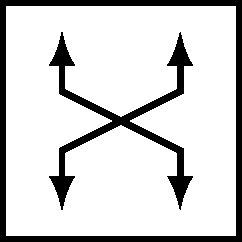
\includegraphics[width=0.9cm]{../common/fig-switch.pdf}
}
\providecommand{\router}{%
    
\includegraphics[width=0.9cm]{../common/fig-router.pdf}
}

\begin{frame}[label=noBackwardsQ]{aside: no backwards broadcast}
    \begin{itemize}
    \item recall: broadcast sent to all but incoming port
    \item question: what would happen if we didn't do this?
        \begin{itemize}
        \item multiple may apply
        \end{itemize}
    \end{itemize}
\begin{tabular}{l}
A. might cause host to receive duplicates \\
B. might cause copies sent to non-incoming port to be dropped \\
C. might cause frames sent at same time to be dropped \\
D. might cause frames sent much later to be dropped \\
\end{tabular}
\end{frame}

\begin{frame}[fragile]{loop from backwards broadcast}
\begin{tikzpicture}[remember picture]
\tikzset{
    computer/.style={inner sep=0mm,outer sep=0mm,execute at begin node={\computer}},
    switch/.style={inner sep=0mm,outer sep=0mm,execute at begin node={\switch}},
    connect/.style={draw,very thick,Latex-Latex},
    connect big/.style={draw,ultra thick,Latex-Latex},
    port/.style={pos=0.95,fill=white,circle,draw,inner sep=0mm},
    port beginning/.style={pos=0.05,fill=white,circle,draw,inner sep=0mm},
    mac label/.style={
        draw,fill=white,inner sep=1mm,font=\tiny\tt,
    },
    one packet/.style n args={3}{
        alt={<#1>{
            postaction=decorate,
            decoration={
                markings,
                mark={at position .5 with
                    \node[
                        thin,transform shape,draw,
                        preaction={fill=white},
                        pattern=crosshatch,pattern color=blue!50,font=\tt,#2
                    ]{#3};
                }
            }
        }},
    },
    one packet forward/.style 2 args={
        one packet={#1}{#2}{>>>},
    },
    one packet backward/.style 2 args={
        one packet={#1}{#2}{<<<},
    },
    hilite/.style={
        alt=<#1>{preaction={fill=red!20},pattern=none},
    },
}
\node[overlay,anchor=north east] at ([xshift=-1cm]current page.north east) {
    time step \myemph{\large\insertoverlaynumber}
};
\foreach \x/\d/\mc/\dir in {15/8cm/AA/north,45/3cm/BB/north,90/2cm/CC/north,135/3cm/DD/north,180/4cm/EE/north,300/4cm/FF/south} {
    \node[computer,label={[mac label,]\dir:00:11:22:33:44:\small\mc},alias=c-\mc] (c-\x) at (\x:\d) {};
}
\node[switch] (s1) at (4,-0.5) {};
\node[switch] (s2) at (-1,-2.5) {};
\draw[connect,one packet forward=1,one packet backward={2}{hilite=2}] (c-15) -- (s1) node[port] {1};
\draw[connect,one packet backward=2,one packet backward=4] (c-45) -- (s1) node[port] {2};
\draw[connect,one packet backward=2,one packet backward=4] (c-300) -- (s1) node[port] {3};
\draw[connect,one packet backward=3] (c-90) -- (s2) node[port] {2};
\draw[connect,one packet backward=3] (c-135) -- (s2) node[port] {3};
\draw[connect,one packet backward=3] (c-180) -- (s2) node[port] {4};
\draw[connect big,one packet forward=2,one packet backward={3}{hilite=3},one packet forward={4}{hilite=4}] (s1) -- (s2) node[port beginning] {4} node [port] {1};
\end{tikzpicture}
\end{frame}

\begin{frame}{loops}
    \begin{itemize}
    \item each packet keeps getting sent indefinitely
    \item remember: happens for \textit{every packet sent}
    \item quickly overwhelms link between switches
    \vspace{.5cm}
    \item but can just avoid by not sending back?
    \end{itemize}
\end{frame}

\begin{frame}[fragile]{loops with only-to-other}
\begin{tikzpicture}[remember picture]
\tikzset{
    computer/.style={inner sep=0mm,outer sep=0mm,execute at begin node={\computer}},
    switch/.style={inner sep=0mm,outer sep=0mm,execute at begin node={\switch}},
    connect/.style={draw,very thick,Latex-Latex},
    connect big/.style={draw,ultra thick,Latex-Latex},
    port/.style={pos=0.95,fill=white,circle,draw,inner sep=0mm},
    port beginning/.style={pos=0.05,fill=white,circle,draw,inner sep=0mm},
    mac label/.style={
        draw,fill=white,inner sep=1mm,font=\tiny\tt,
    },
    one packet/.style n args={3}{
        alt={<#1>{
            postaction=decorate,
            decoration={
                markings,
                mark={at position .5 with
                    \node[
                        thin,transform shape,draw,
                        preaction={fill=white},
                        pattern=crosshatch,pattern color=blue!50,font=\tt,#2
                    ]{#3};
                }
            }
        }},
    },
    two packet/.style n args={3}{
        alt={<#1>{
            postaction=decorate,
            decoration={
                markings,
                mark={at position .3 with
                    \node[
                        thin,transform shape,draw,
                        preaction={fill=white},
                        pattern=crosshatch,pattern color=blue!50,font=\tt,#2
                    ]{#3};
                },
                mark={at position .6 with
                    \node[
                        thin,transform shape,draw,dashed,
                        preaction={fill=white},
                        pattern=crosshatch,pattern color=blue!50,font=\tt,#2
                    ]{#3};
                }
            }
        }},
    },
    one packet forward/.style 2 args={
        one packet={#1}{#2}{>>>},
    },
    one packet backward/.style 2 args={
        one packet={#1}{#2}{<<<},
    },
    one packet both/.style 2 args={
        one packet={#1}{#2}{<</>>},
    },
    hilite/.style={
        alt=<#1>{preaction={fill=red!20},pattern=none},
    },
    hilite b/.style={
        alt=<#1>{dashed,preaction={fill=red!20},pattern=none},
    },
    hilite alt/.style={
        alt=<#1>{pattern=north west lines,pattern color=black!50},
    },
}
\node[overlay,anchor=north east] at ([xshift=-1cm]current page.north east) {
    time step \myemph{\large\insertoverlaynumber}
};
\foreach \x/\d/\mc/\dir in {15/8cm/AA/north,30/4cm/BB/north,90/2cm/CC/north,135/3cm/DD/north,180/4cm/EE/north,46/2cm/FF/north} {
    \node[computer,label={[mac label,]\dir:00:11:22:33:44:\small\mc},alias=c-\mc] (c-\x) at (\x:\d) {};
}
\node[switch] (s1) at (2.5,-0.5) {};
\node[switch] (s2) at (-1,-0.5) {};
\node[switch] (s3) at (6,-3.5) {};
\draw[connect,one packet forward=1,two packet={5}{}{<<<}] (c-15) -- (s3);
\draw[connect,one packet backward=2,two packet={5}{}{<<<}] (c-BB) -- (s3);
\draw[connect,one packet backward=3,
      one packet backward={4}{hilite alt=4},
      ] (c-FF) -- (s1);
\draw[connect,one packet backward=3,
      one packet backward={4}{hilite alt=4},
      ] (c-90) -- (s2);
\draw[connect,one packet backward=3,
      one packet backward={4}{hilite alt=4},
     ] (c-135) -- (s2);
\draw[connect,one packet backward=3,
      one packet backward={4}{hilite alt=4},
      ] (c-180) -- (s2);
\draw[connect big,one packet both={3}{hilite=3},] (s1) -- (s2);
\draw[connect big,one packet backward=2,one packet forward={4}{hilite b=4},
    one packet backward={5}{hilite=5}] (s1) -- (s3);
\draw[connect big,one packet backward={2}{hilite=2},
    one packet forward={4}{hilite=4},
    one packet backward={5}{hilite b=5}] (s2) -- (s3);
\end{tikzpicture}
\end{frame}



\section{preview: internetworks}

\begin{frame}{preview: routing}
    \begin{itemize}
    \item better ways to decide where to send packets
    \item \ldots but require coordinating between switches
        \begin{itemize}
        \item avoid loops
        \item choose between multiple paths
        \item avoid `flooding' for each new machine
        \end{itemize}
    \vspace{.5cm}
    \item problem also very important for large networks\ldots
    \item \ldots like the Internet
    \item we will revisit it when we talk about IP routing
    \end{itemize}
\end{frame}


\section{IP addresses}

\subsection{IPv4}

\subsubsection{address format}
\begin{frame}{IPv4 addresses}
    \begin{itemize}
    \item 32-bit numbers
    \item typically written like 128.143.67.11
        \begin{itemize}
        \item four 8-bit decimal values separated by dots
        \item first part is most significant
        \item same as $128\cdot 256^3+143\cdot 256^2 + 67\cdot256 + 11 = 2\,156\,782\,459$
        \end{itemize}
    \end{itemize}
\end{frame}


\subsubsection{CIDR notation}
\begin{frame}{IPv4 address blocks}
\begin{itemize}
    \item often will want to talk about group of IPv4 addresses
    \item example: {\color<2>{violet!70!black}128.143.67.64}---{\color<2>{green!70!black}128.143.67.127} (inclusive)
    \item<2-> {\tt\color<2>{violet!70!black}\myemph<3>{10000000 10001111 01000011 001}\myemph<4>{00000}}
    \item<2-> {\tt\color<2>{green!70!black}\myemph<3>{10000000 10001111 01000011 001}\myemph<4>{11111}}
    \item<3-> first 27 bits always same; anything for last bits
    \item<5-> more convenient representation: 128.143.67.64/27
    \item<5-> called ``CIDR notation''
        \begin{itemize}
        \item CIDR = classless inter-domain routing (will come up when we discuss routing)
        \end{itemize}
\end{itemize}
\end{frame}

\begin{frame}{CIDR notation examples}
    \begin{itemize}
    \item 5.7.3.3/14 = 5.4.0.0/14 = 5.4.0.0---5.7.255.255
        \begin{itemize}
        \item<2-> \myemph<2>{also written 5.4/14}
        \end{itemize}
    \item 128.143.0.0/16 =  128.143.0.0---128.143.255.255
        \begin{itemize}
        \item<2-> \myemph<2>{also written 128.143/16}
        \end{itemize}
    \item 192.168.0.0/24 =  192.168.0.0---192.168.0.255
    \item 10.0.0.0/8 = 10.0.0.0--10.255.255.255
        \begin{itemize}
        \item<2-> \myemph<2>{also written 10/8}
        \end{itemize}
    \end{itemize}
\end{frame}

\begin{frame}{alternate notation: netmasks}
    \begin{itemize}
    \item instead of writing 128.143.67.64/27 might say
    \item 128.143.67.64 and ``network mask'' of 255.255.255.224
    \item 255.255.255.224 = 27 1's
    \vspace{.5cm}
    \item<2-> if some-address bitwise-AND netmask = 128.143.67.64 bitwise-AND netmask, \\
        then some-address is in the range
    \end{itemize}
\end{frame}


\subsection{IPv6}
\begin{frame}{IPv6 addresses}
    \begin{itemize}
    \item IPv6 like IPv4, but with 128-bit numbers
    \item written in hex, 16-bit parts, seperated by colons (\texttt{:})
    \item strings of 0s represented by double-colons (\texttt{::})
    \item typically given to users in blocks of $2^{80}$ or $2^{64}$ addresses
    \vspace{.5cm}
    \item \fontsize{10}{11}\selectfont\texttt{2607:f8b0:400d:c00::6a} = \\
          \texttt{2607:f8b0:400d:0c00:0000:0000:0000:006a}
          \begin{itemize}
          \item \texttt{2607f8b0400d0c0000000000000006a}$_\text{SIXTEEN}$
          \end{itemize}
    \end{itemize}
\end{frame}

\begin{frame}{IPv6 CIDR notation examples}
    \begin{itemize}
    \item 2607:fb80:400d:0c00::/64 = 
        \begin{itemize}
        \item \texttt{2607:fb80:400d:0c00:0000:0000:0000:0000}---\\
              \texttt{2607:fb80:400d:0c00:ffff:ffff:ffff:ffff}
        \end{itemize}
    \item 2607:fb80::/30 = 
        \begin{itemize}
        \item \texttt{2607:fb80:0000:0000:0000:0000:0000:0000}---\\
              \texttt{2607:fb83:ffff:ffff:ffff:ffff:ffff:ffff}
        \end{itemize}
    \end{itemize}
\end{frame}


\subsection{address space allocation}
\begin{frame}{}
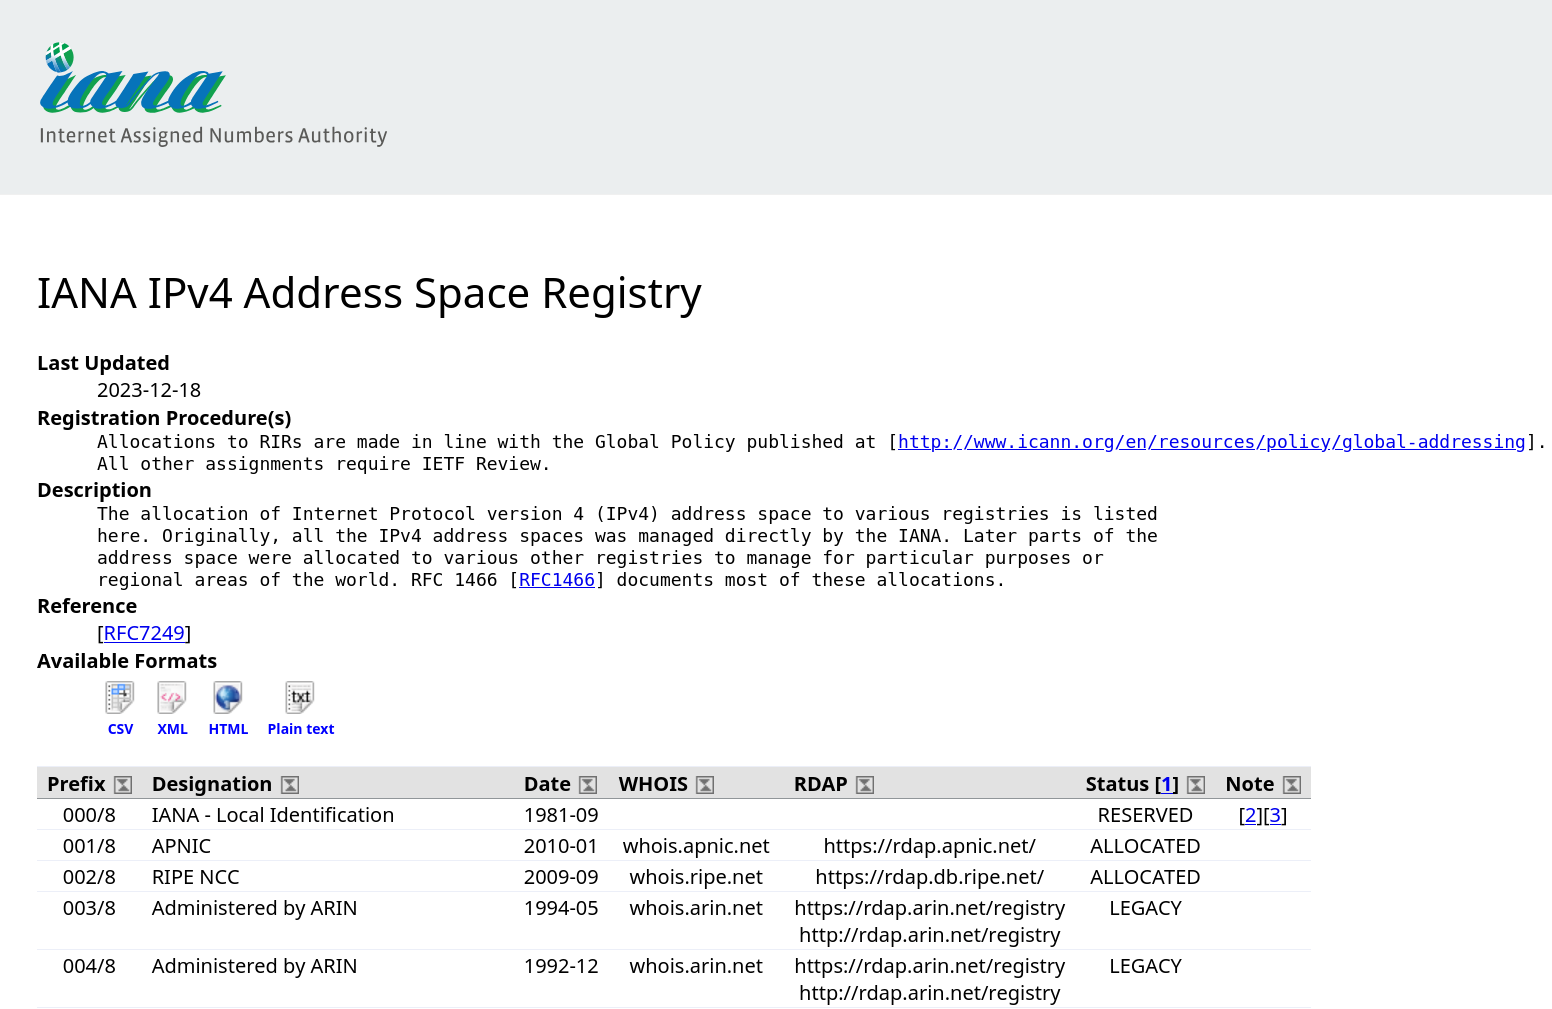
\includegraphics[width=\textwidth]{../arp/iana-registry-screenshot}
\end{frame}

\begin{frame}{}
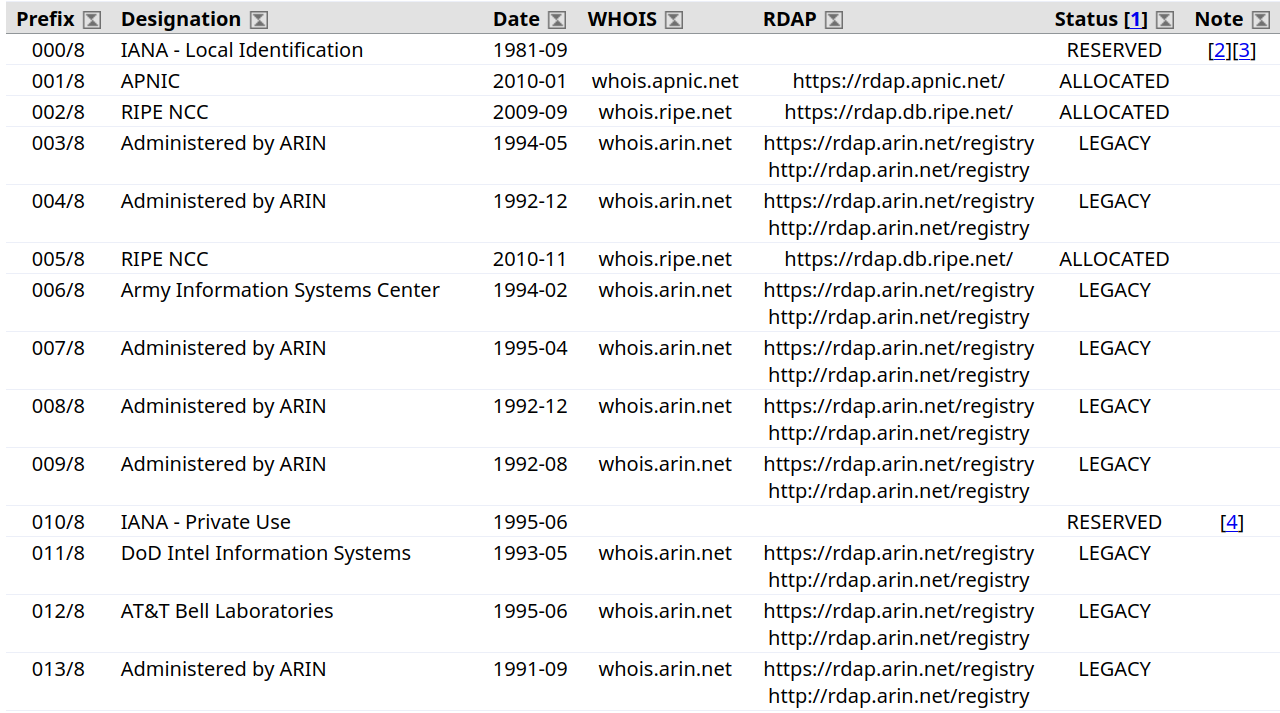
\includegraphics[width=\textwidth]{../arp/iana-ipv4-allocs}
(and 241 more)
\end{frame}

\begin{frame}[fragile]{}
\begin{tikzpicture}
\node (v6 space top) {
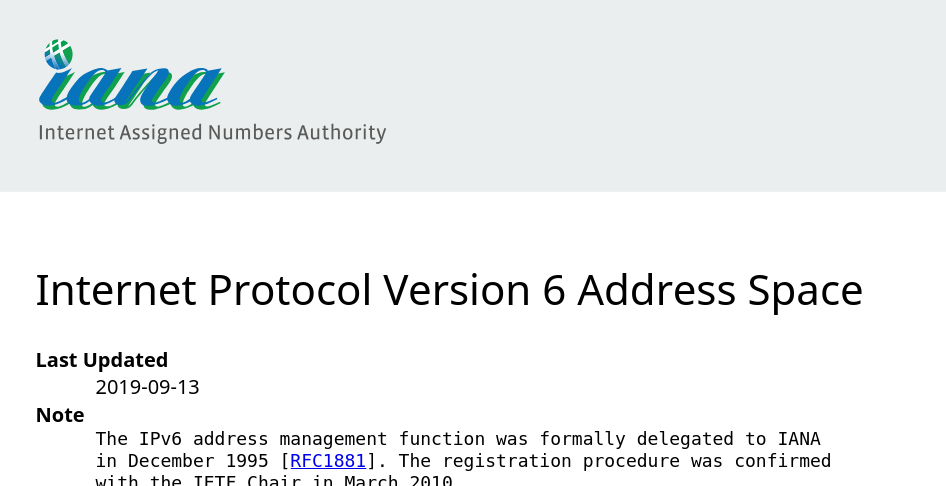
\includegraphics[width=8cm]{../arp/iana-v6-addr-top} 
};
\node[anchor=north,font=\Huge,inner sep=1mm] (v6 space ldots) at ([yshift=-1mm]v6 space top.south) {\ldots};
\node[anchor=north] at (v6 space ldots.north) {
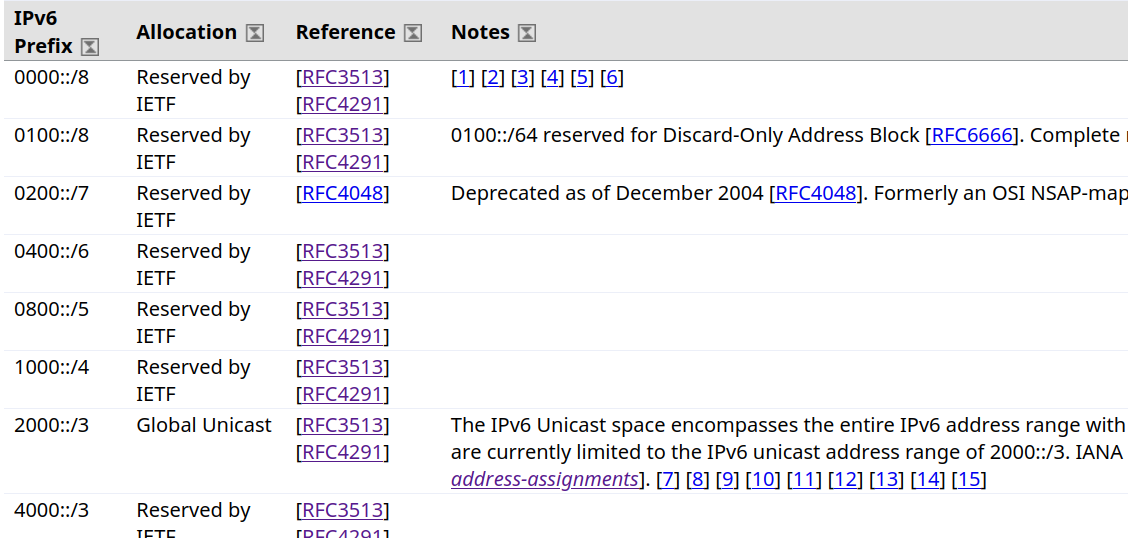
\includegraphics[width=8cm]{../arp/iana-v6-addr-bottom2}
};
\node[anchor=north west] at (v6 space top.north east) {
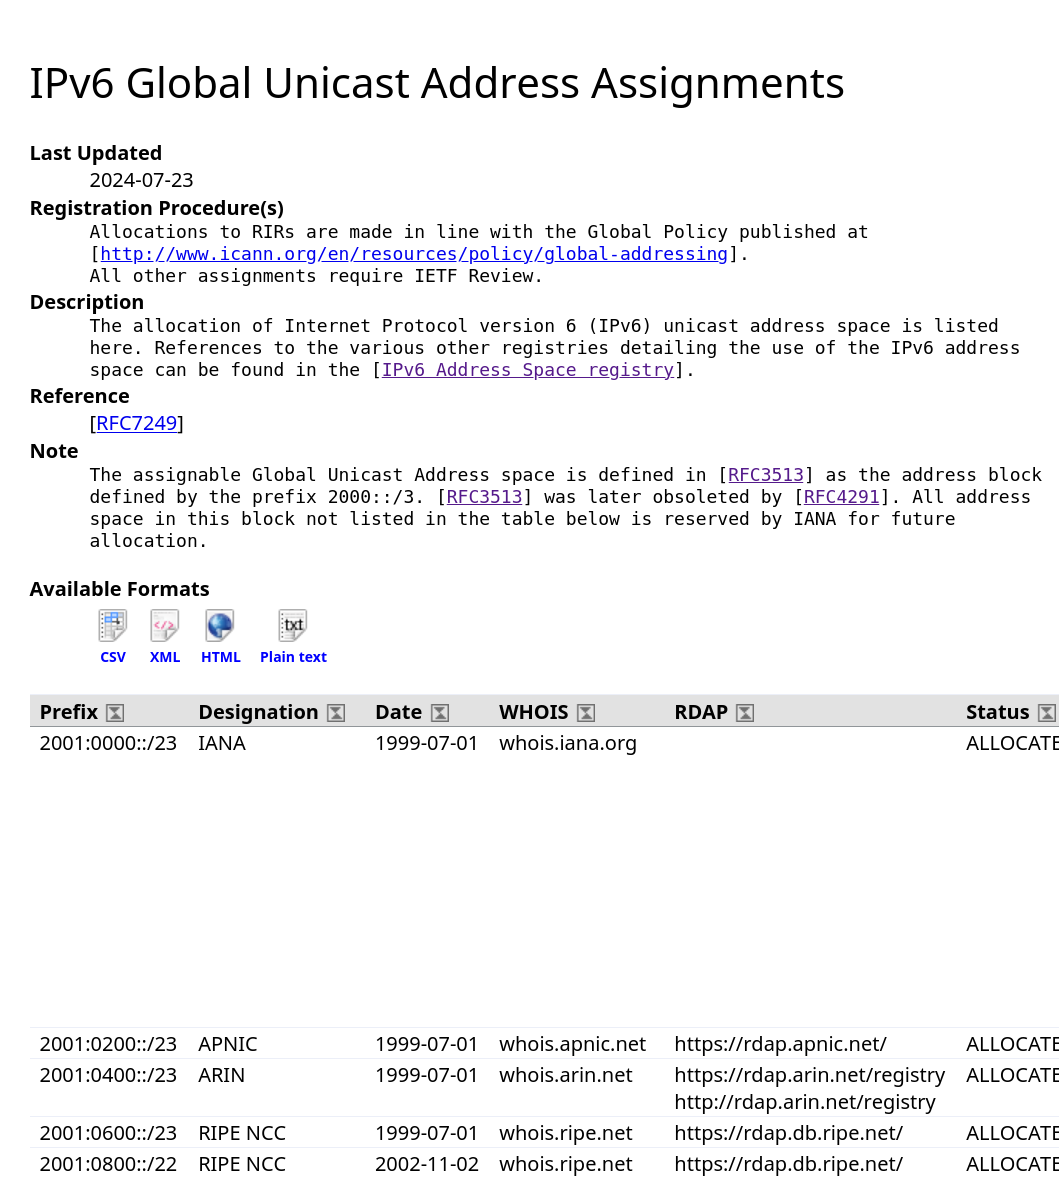
\includegraphics[width=8cm]{../arp/iana-v6-unicast}
};
\end{tikzpicture}
\end{frame}

\begin{frame}{regional internet registries (RIRs)}
\begin{tikzpicture}
\node[inner sep=1mm] (rir) {
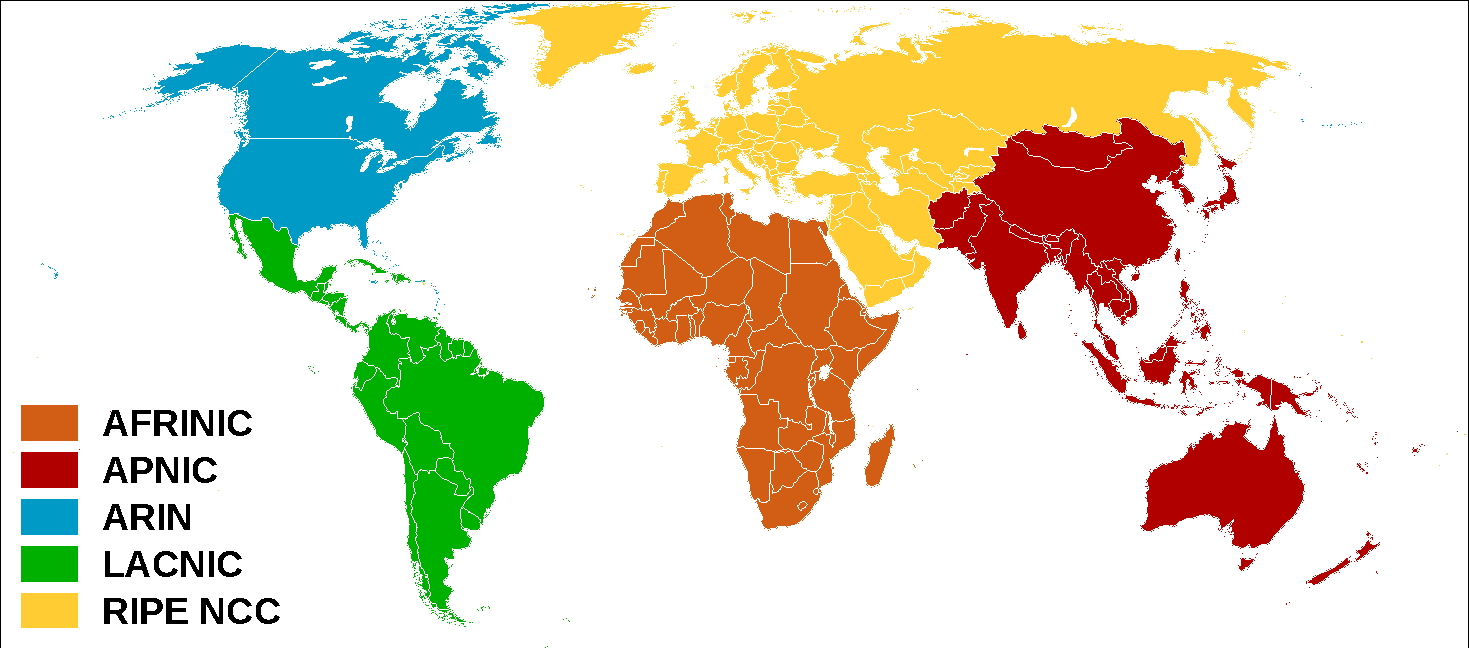
\includegraphics[height=0.35\textheight]{Regional_Internet_Registries_world_map.pdf} 
};
\node[align=left,anchor=north west,font=\scriptsize] at (rir.north east) {
map from Wikimedia Commons, \\
users Dork, Canuckguy et al, S\'emhur, CC-BY-SA 3.0
};
\end{tikzpicture}
\begin{itemize}
\item most useful addresses managed by RIRs
    \begin{itemize}
    \item African Network Information Centre (AFRINIC)
    \item American Registry for Internet Numbers (ARIN)
    \item Asia Pacific Network Information Centre (APNIC)
    \item Latin American and Carribean Network Information Centre (LACNIC)
    \item R\'eseaux IP Europ\'eens Network Coordination Centre (RIPE NCC)
    \end{itemize}
\end{itemize}
\end{frame}

\begin{frame}{RIR suballocations}
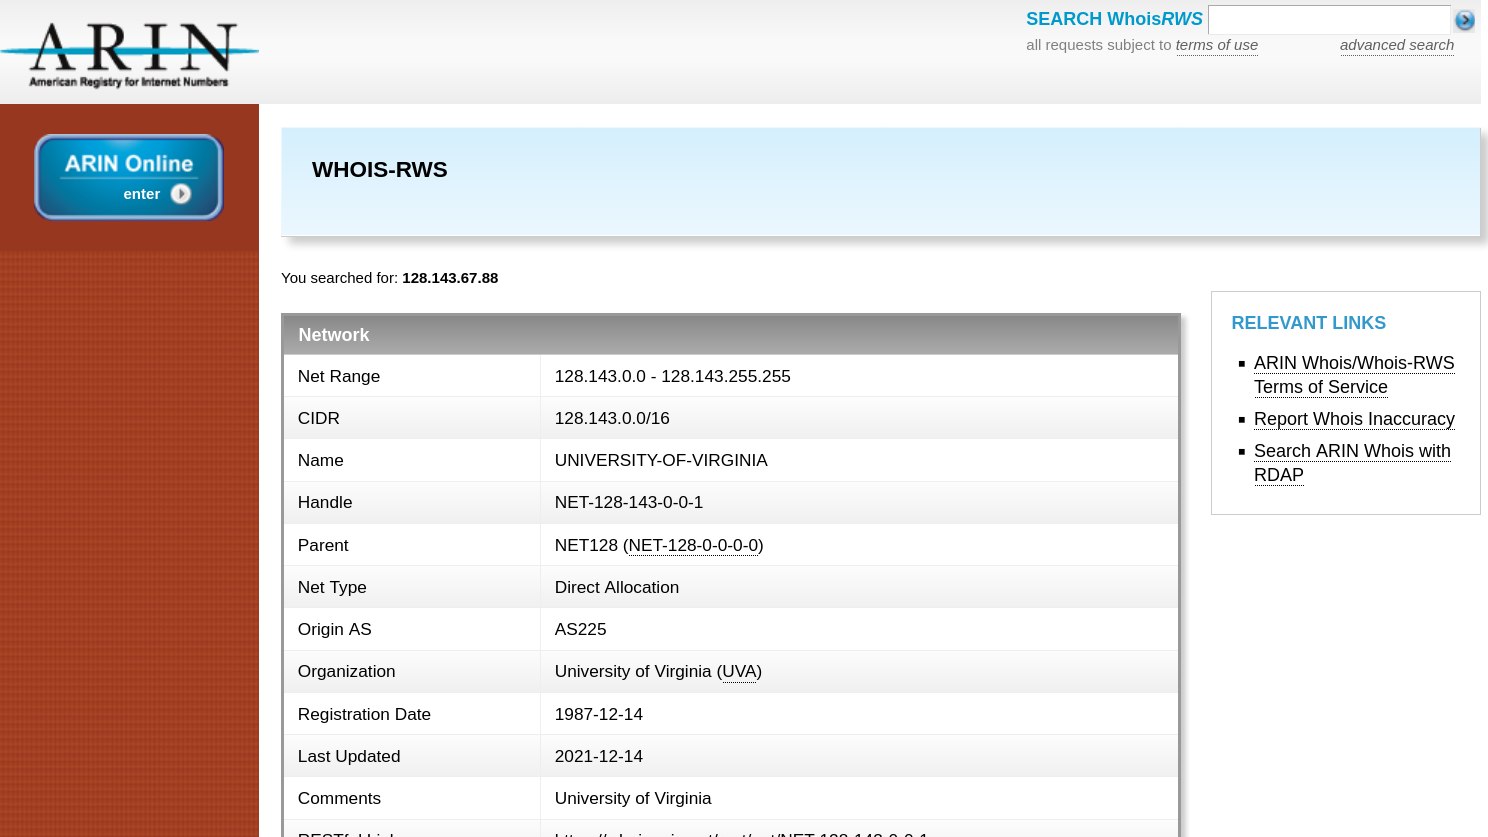
\includegraphics[width=\textwidth]{../arp/arin-whois-virginia}
\end{frame}

\begin{frame}{special IPv4 addresses}
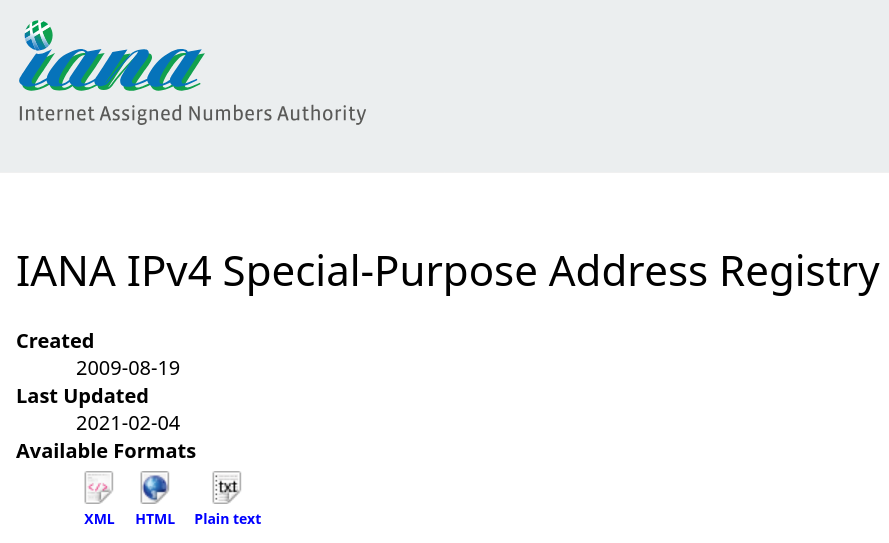
\includegraphics[width=\textwidth]{../arp/iana-special-ipv4-header}
\end{frame}

\begin{frame}{special IPv4 addresses}
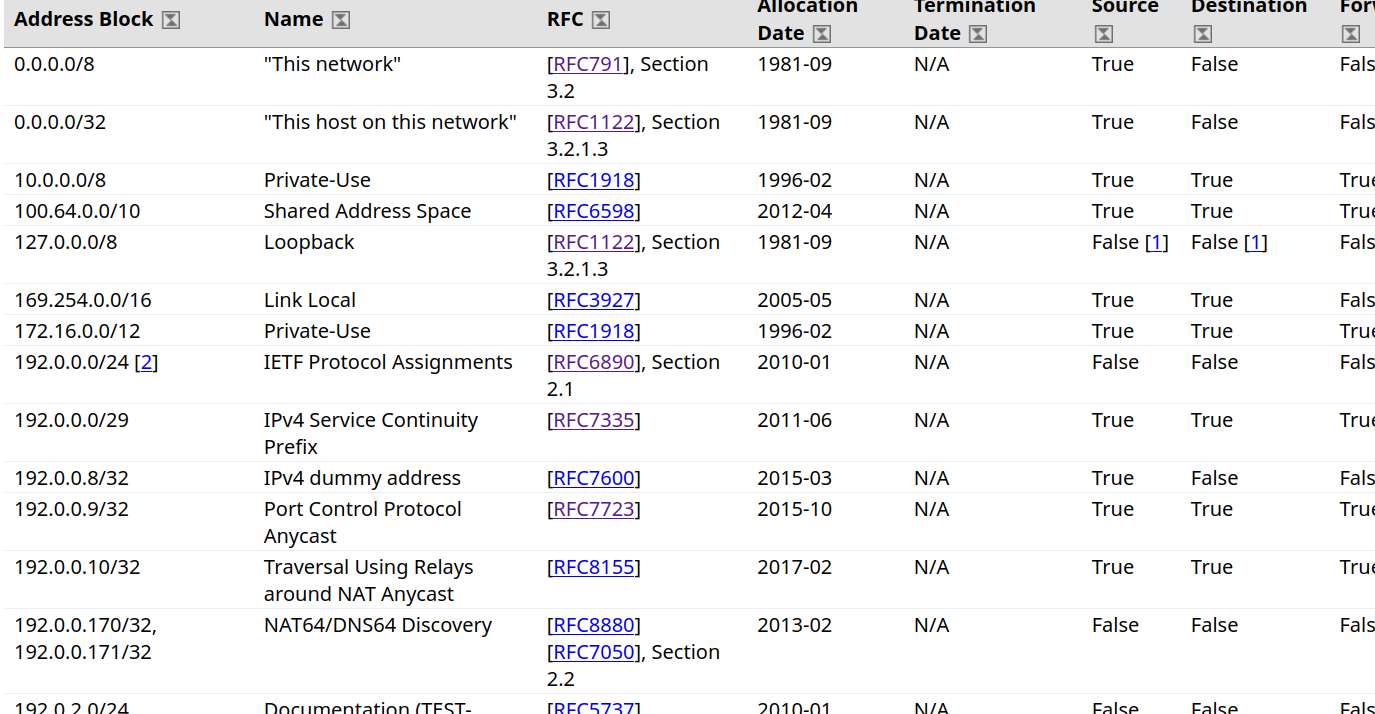
\includegraphics[width=\textwidth]{../arp/iana-special-ipv4-detail}
\end{frame}

\begin{frame}{selected special IP addresses}
\begin{itemize}
\item loopback (current machine) --- {\tt 127/8} (v4), {\tt ::1/128} (v6)
\item link-local (current network only) ---
    \begin{itemize}
    \item {\tt 169.254/16} (v4), {\tt ff80::/10} (v6)
    \end{itemize}
\item private use (non-public networks only) --- \\
    \begin{itemize}
    \item {\tt 192.168/16}, {\tt 172.16/12}, {\tt 10/8} (v4), (kinda) {\tt fc00::/7} (v6)
    \end{itemize}
\item multicast groups and related --- {\tt 224/4} (v4), {\tt ff00::/8} (v6)
    \begin{itemize}
    \item multiple nodes can be part of a single ``multicast group''
    \end{itemize}
\item broadcast (all on current network) --- 
    \begin{itemize}
    \item {\tt 255.255.255.255}, {\tt ff01::1}
    \end{itemize}
\item ``future use'' --- 
    \begin{itemize}
    \item rest of {\tt 240/4} (v4), {\tt 4000::}---{\tt efff::} (v6)
    \end{itemize}
\end{itemize}
\end{frame}


\subsection{which link-local addresses}
\begin{frame}{which link local?}
    \begin{itemize}
    \item ``link local'': \texttt{169.254/16}, \texttt{fe80::/10}
    \item specific to each local network
    \vspace{.5cm}
    \item \texttt{fe80::17} on network A != \texttt{fe80::17} on network B
    \vspace{.5cm}
    \item problem: machine can be connected to two networks
    \item<2-> solution: \texttt{fe80::17\%A} versus \texttt{fe80::17\%B}
    \item<3-> what about IPv4? uh... too bad?
        \begin{itemize}
        \item ``There is no standard or obvious solution to this problem\ldots
        must be done explicitly through other means. The specification does not stipulate
        those means.'' --- RFC 3927, section 3.2
        \end{itemize}
    \end{itemize}
\end{frame}



\section{routing versus switching}
\subsection{tables}
\usetikzlibrary{fit,matrix}
\usetikzlibrary{arrows.meta,calc,shapes}
\providecommand{\computer}{%
    
\includegraphics[width=1cm]{../common/Noun_project_216.pdf}
}
\providecommand{\switch}{%
    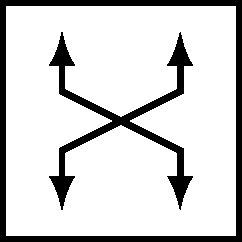
\includegraphics[width=0.9cm]{../common/fig-switch.pdf}
}
\providecommand{\router}{%
    
\includegraphics[width=0.9cm]{../common/fig-router.pdf}
}
\begin{frame}{switch v router: tables}
\begin{tikzpicture}
\matrix[tight matrix,
    nodes={minimum height=.6cm},
    column 1/.style={nodes={text width=5cm,font=\small\tt}},
    column 2/.style={nodes={text width=1cm,font=\small\tt}},
    row 1/.style={nodes={font=\small}},
    label={north:switch (`bridge') table},
] (bridge table) {
MAC address \& port \\
00:11:22:33:44:55 \& 1 \\
00:33:00:01:02:aa \& 2 \\
00:44:00:01:02:bb \& 3 \\
\ldots \& \ldots \\
\normalfont default \& (all) \\
};
\matrix[tight matrix,
    nodes={minimum height=.6cm},
    column 1/.style={nodes={text width=4.5cm,font=\small\tt}},
    column 2/.style={nodes={text width=2cm,font=\small\tt,alt=<4>{fill=red!10}}},
    column 3/.style={nodes={text width=1cm,font=\small\tt,alt=<3>{fill=red!10}}},
    row 1/.style={nodes={font=\small}},
    label={north:routing table},
    anchor=north west
] (route table) at ([xshift=.5cm]bridge table.north east){
IP addresses \& gateway \& iface \\
2001:0db8:40::/48 \& --- \& int \\
3fff:1000:19::/48 \& --- \& ext \\
\ldots \& \ldots \& \ldots \\
\normalfont default \& fe80::17 \& ext \\
};
\begin{visibleenv}<2>
\node[
    draw=red,ultra thick,fit=(bridge table),
] (bridge table around) {};
\node[align=left,anchor=north west] at (bridge table around.south west) {
    one logical device with multiple ports \\
    not in table: always broadcast
};
\end{visibleenv}
\begin{visibleenv}<3->
\node[
    draw=red,ultra thick,fit=(route table),
] (route table around) {};
\end{visibleenv}
\begin{visibleenv}<3>
\node[align=left,anchor=north] at (route table around.south) {
    `interface' = which network \\
    ~ \\
    one interface might have multiple ports \\
    that are `bridged' together \\
};
\end{visibleenv}
\begin{visibleenv}<4>
\node[align=left,anchor=north] at (route table around.south) {
    gateway = who to send to next \\
    no gateway = `direct' to destination \\
    ~ \\
    need to have specific destination \\
    to send to on interface
};
\end{visibleenv}
\end{tikzpicture}
\end{frame}

\begin{frame}{trivial tables}
\begin{itemize}
\item let's say we're connected to ONE interface with ONE port
\item<2-> tables are really trivial:
\end{itemize}
\begin{visibleenv}<2->
\begin{tikzpicture}
\matrix[tight matrix,
    nodes={minimum height=.6cm},
    column 1/.style={nodes={text width=2.5cm,font=\small}},
    column 2/.style={nodes={text width=1.5cm,font=\small}},
    row 1/.style={nodes={font=\small}},
    label={north:switch (`bridge') table},
] (bridge table) {
MAC address \& port \\
default \& the port \\
};
\matrix[tight matrix,
    nodes={minimum height=.6cm},
    column 1/.style={nodes={text width=4.5cm,font=\small\tt}},
    column 2/.style={nodes={text width=2.5cm,font=\small\tt,alt=<4>{fill=red!10}}},
    column 3/.style={nodes={text width=2.5cm,font=\fontsize{9}{10}\tt,alt=<3>{fill=red!10}}},
    row 1/.style={nodes={font=\small}},
    label={north:routing table (IPv6)},
    anchor=north west
] (route table) at ([xshift=.5cm]bridge table.north east){
IP addresses \& gateway \& iface \\
2001:0db8:40::/48 \& --- \& the interface \\
\normalfont default \& fe80::17 \& the interface \\
};
\matrix[tight matrix,
    nodes={minimum height=.6cm},
    column 1/.style={nodes={text width=4.5cm,font=\small\tt}},
    column 2/.style={nodes={text width=2.5cm,font=\small\tt,alt=<4>{fill=red!10}}},
    column 3/.style={nodes={text width=2.5cm,font=\fontsize{9}{10}\tt,alt=<3>{fill=red!10}}},
    row 1/.style={nodes={font=\small}},
    label={north:routing table (IPv4)},
    anchor=north west,
] (route table v4) at ([yshift=-.8cm]route table.south west){
IP addresses \& gateway \& iface \\
192.0.2.0/24 \& --- \& the interface \\
\normalfont default \& 192.0.2.1 \& the interface \\
};
\end{tikzpicture}
\end{visibleenv}
\end{frame}


\subsection{tables}
\usetikzlibrary{fit,matrix}
\usetikzlibrary{arrows.meta,calc,shapes}
\providecommand{\computer}{%
    
\includegraphics[width=1cm]{../common/Noun_project_216.pdf}
}
\providecommand{\switch}{%
    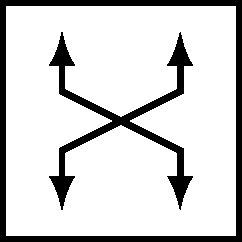
\includegraphics[width=0.9cm]{../common/fig-switch.pdf}
}
\providecommand{\router}{%
    
\includegraphics[width=0.9cm]{../common/fig-router.pdf}
}

\begin{frame}{switch v router: on the wires}
\begin{tikzpicture}
\tikzset{
    computer/.style={inner sep=0mm,outer sep=0mm,execute at begin node={\computer}},
    switch/.style={inner sep=0mm,outer sep=0mm,execute at begin node={\switch}},
    router/.style={inner sep=-1mm,outer sep=0mm,execute at begin node={\router},circle},
    connect/.style={draw,very thick,Latex-Latex},
    connect big/.style={draw,ultra thick,Latex-Latex},
    addr label/.style={align=left,font=\fontsize{9}{10}\selectfont\tt},
}
\node[computer,label={[addr label]south:MAC 00:\ldots:AA\\IP 10.0.1.2},alt=<5>{draw=red,ultra thick,fill=red!10}] (n1-c1) at (0, -2.5) {};
\node[computer,label={[addr label]south:MAC 04:\ldots:BB\\IP 10.0.1.3}]  (n1-c2) at (0, 0) {};
\node[switch] (n1-s1) at (3,-1) {};
\node[switch] (n1-s2) at (5,-4) {};
\node[computer,label={[addr label]south:MAC 05:\ldots:CC\\IP 10.0.1.4}] (n1-c3) at (1, -5) {};
\draw[connect] (n1-c1) -- (n1-s1);
\draw[connect] (n1-c2) -- (n1-s1);
\draw[connect] (n1-c3) -- (n1-s2);
\draw[connect big] (n1-s1) -- (n1-s2);
\node[router,label={[addr label]south:MAC \myemph<5-6>{02:\ldots:DD} / 02:\ldots:DE\\IP: 10.0.1.1 / 10.0.2.15},alt=<5-6>{fill=red!10,draw=red,ultra thick}] (n1n2) at (9, -5) {};
\node[switch] (n2-s1) at (11, -3) {};
\node[computer,label={[addr label]south:MAC 03:\ldots:EE\\IP: \myemph<5>{10.0.2.2}},alt=<5>{draw=red,ultra thick,fill=red!10}] (n2-c1) at (12.5, -4) {};
\draw[connect](n2-s1) -- (n2-c1);

\draw[connect big] (n1-s2) -- (n1n2);
\draw[connect big] (n2-s1) -- (n1n2);
\begin{pgfonlayer}{bg}
    \begin{visibleenv}<2->
        \path[overlay,draw=violet,fill=violet!10]
            (-1.3, -7) -- (5, -7) -- (9, -7) -- (9, -3) -- (4, .75) -- (-1.3, .75) -- cycle;
        \path[overlay,draw=green,fill=green!10]
            (7, 0) -- (8, -2) -- (9, -3) -- (9, -7) -- (13.5, -7) -- (13.5, 0) -- cycle;
        \node[anchor=south,font=\tt] at (5, -7) {10.0.1.0/24};
        \node[anchor=south,font=\tt] at (11, -7) {10.0.2.0/24};
    \end{visibleenv}
\end{pgfonlayer}
\begin{visibleenv}<3->
        \foreach \x [remember=\x as \lastx (initially n1-c1)] in {n1-s1,n1-s2,n1n2,n2-s1,n2-c1} {
            \path[draw,dotted,blue,line width=1mm,arrows=-Latex] (\lastx) -- (\x);
        }
\end{visibleenv}
\begin{visibleenv}<4->
    \path[draw,blue,thick] ($(n1-c1)!0.5!(n1-s1)$) -- (3.7, -1) ++ (0, 1.) coordinate (n1 frame base);
    \node[font=\fontsize{9}{10}\tt,anchor=north west] (n1 outer) at (n1 frame base) {
        00:\ldots:AA\hspace{1mm}$\rightarrow$\myemph<5>{\hspace{1mm}02:\ldots:DD}
    };
    \node[align=left,font=\fontsize{9}{10}\tt,anchor=north west,draw=black!50,very thick,
          alt=<6>{fill=red!10},
    ] (n1 inner) at ([xshift=1mm]n1 outer.south west) {
        10.0.1.3 $\rightarrow$ \myemph<5>{10.0.2.2} \\
        (actual data)
    };
    \path (12, -0) ++ (-2.25, 0.5) coordinate (n2 frame base);
    \node[font=\fontsize{9}{10}\tt,anchor=north west] (n2 outer) at (n2 frame base) {
        02:\ldots:DE\hspace{1mm}$\rightarrow$\hspace{1mm}03:\ldots:EE
    };
    \node[align=left,font=\fontsize{9}{10}\tt,anchor=north west,draw=black!50,very thick,
          alt=<6>{fill=red!10}
    ] (n2 inner) at ([xshift=1mm]n2 outer.south west) {
        10.0.1.3 $\rightarrow$ 10.0.2.2 \\
        (actual data)
    };
\end{visibleenv}
\begin{pgfonlayer}{bg}
    \begin{visibleenv}<4->
    \node[inner sep=0mm,fill=white,draw=blue,very thick,
          fit={(n1 outer) (n1 inner) ([yshift=-1mm]n1 inner.south) ([xshift=1mm]n1 inner.east)}
    ] (n1 box) {};
    \path[draw,blue,thick] ($(n1-s1)!0.5!(n1-s2)$) -- (n1 box);
    \path[draw,blue,thick] ($(n1-s2)!0.5!(n1n2)$) -- (n1 box);
    \node[inner sep=0mm,fill=white,draw=blue,very thick,
          fit={(n2 outer) (n2 inner) ([yshift=-1mm]n2 inner.south) ([xshift=1mm]n2 inner.east)}
    ] (n2 box) {};
    \path[draw,blue,thick] ($(n2-s1)!0.5!(n1n2)$) -- ([xshift=.5cm]n2 box.south west);
    \path[draw,blue,thick] ($(n2-c1)!0.5!(n2-s1)$) -- ([xshift=2cm]n2 box.south west);
    \end{visibleenv}
\end{pgfonlayer}
\begin{visibleenv}<5>
    \node[fill=white,draw=red,ultra thick,align=left] at (3, -5) {
        MAC address = on \textit{local} network \\
        IP address = somewhere else
    };
\end{visibleenv}
\begin{visibleenv}<7>
    \draw[red, ultra thick] (n1 inner) -- (n2 inner)
        node[inner sep=0mm,
             midway,pin={[pin edge={red,ultra thick},fill=white,draw=red,thick,align=center]-90:IP packet copied as is\\placed in new frame}] {};
\end{visibleenv}
% FIXME:    show packets involved
% FIXME:    show frames involved
% FIXME:    show bridge/routing table
\end{tikzpicture}
\end{frame}

\begin{frame}{steps at the sender}
\begin{tikzpicture}
\tikzset{
    computer/.style={inner sep=0mm,outer sep=0mm,execute at begin node={\computer}},
    switch/.style={inner sep=0mm,outer sep=0mm,execute at begin node={\switch}},
    router/.style={inner sep=-1mm,outer sep=0mm,execute at begin node={\router},circle},
    connect/.style={draw,very thick,Latex-Latex},
    connect big/.style={draw,ultra thick,Latex-Latex},
    addr label/.style={align=left,font=\fontsize{9}{10}\selectfont\tt},
}
\node[computer,label={[addr label]south:MAC 00:\ldots:AA\\IP 10.0.1.2},alt=<2->{draw=red,ultra thick,fill=red!10}] (n1-c1) at (0, -2.5) {};
\node[font=\bfseries] at (n1-c1) {src};
\node[computer,label={[addr label]south:MAC 04:\ldots:BB\\IP 10.0.1.3}]  (n1-c2) at (0, 0) {};
\node[switch] (n1-s1) at (3,-1) {};
\node[switch] (n1-s2) at (5,-4) {};
\node[computer,label={[addr label]south:MAC 05:\ldots:CC\\IP 10.0.1.4}] (n1-c3) at (1, -5) {};
\draw[connect] (n1-c1) -- (n1-s1);
\draw[connect] (n1-c2) -- (n1-s1);
\draw[connect] (n1-c3) -- (n1-s2);
\node[router,label={[addr label]south:MAC 02:\ldots:DD / 02:\ldots:DE\\IP: 10.0.1.1 / 10.0.2.15}] (n1n2) at (9, -5) {};
\draw[connect big] (n1-s1) -- (n1-s2);
\draw[connect big] (n1-s2) -- (n1n2);
    \foreach \x [remember=\x as \lastx (initially n1-c1)] in {n1-s1,n1-s2,n1n2} {
        \path[draw,dotted,blue,line width=1mm,arrows=-Latex] (\lastx) -- (\x);
    }

    \path (3.7, -1) ++ (0, 1.) coordinate (n1 frame base);
    \begin{visibleenv}<3>
        \node[font=\fontsize{9}{10}\tt,anchor=north west] (n1 outer pre 1) at (n1 frame base) {
            \myemph<4>{00:\ldots:AA}\hspace{1mm}$\rightarrow$\hspace{1mm}???????
        };
    \end{visibleenv}
    \begin{visibleenv}<4>
        \node[font=\fontsize{9}{10}\tt,anchor=north west] (n1 outer pre 2) at (n1 frame base) {
            \myemph<4>{00:\ldots:AA}\hspace{1mm}$\rightarrow$\hspace{1mm}\myemph<4>{\normalfont 10.0.1.1's MAC}
        };
    \end{visibleenv}
    \begin{visibleenv}<5->
        \node[font=\fontsize{9}{10}\tt,anchor=north west] (n1 outer) at (n1 frame base) {
            00:\ldots:AA\hspace{1mm}$\rightarrow$\hspace{1mm}02:\ldots:DD
        };
    \end{visibleenv}
   \begin{visibleenv}<2->
        \node[
            align=left,font=\fontsize{9}{10}\tt,anchor=north west,draw=black!50,very thick,
            alt=<2>{fill=red!10},
        ] (n1 inner) at ([xshift=1mm]n1 outer.south west) {
            10.0.1.2 $\rightarrow$ \myemph<5>{10.0.2.2}\\
            (actual data)
        };
    \end{visibleenv}
    \begin{visibleenv}<2>
        \path[draw=red,ultra thick,arrows=Latex-](n1 inner.east) -- ++(1cm, 0cm) node[right] {
            packet from upper layer
        };
    \end{visibleenv}
    \begin{visibleenv}<3>
        \path[draw=red,ultra thick,arrows=Latex-,align=left] (n1 outer pre 1.east) -- ++(1cm, 0cm) node[right] {
            need to send at link layer
        };
    \end{visibleenv}
    \begin{visibleenv}<4>
        \path[draw=red,ultra thick,arrows=Latex-,align=left] (n1 outer pre 2.east) -- ++(1cm, 0cm) node[right] {
            routing table says: \\
            to 10.0.1.1 \\
            but need MAC address
        };
    \end{visibleenv}
    \begin{visibleenv}<5>
        \path[draw=red,ultra thick,arrows=Latex-,align=left] (n1 outer pre 1.east) -- ++(1cm, 0cm) node[right] {
            need IP:MAC address table \\
            called neighbor table \\
            or ARP table
        };
    \end{visibleenv}
\begin{pgfonlayer}{bg}
    \begin{visibleenv}<3->
    \node[inner sep=0mm,fill=white,draw=blue,very thick,
          fit={(n1 outer) (n1 inner) ([yshift=-1mm]n1 inner.south) ([xshift=1mm]n1 inner.east)}
    ] (n1 box) {};
    \end{visibleenv}
\end{pgfonlayer}
\tikzset{
    route table/.style={
        matrix of nodes,ampersand replacement=\&,
        nodes={execute at begin node={\strut}},
        column 1/.style={nodes={draw,thin,text width=3cm,font=\fontsize{8}{9}\tt,minimum height=0.4cm,inner sep=.1mm}},
        column 2/.style={nodes={draw,thin,text width=2cm,font=\fontsize{8}{9}\tt,minimum height=0.4cm,inner sep=.1mm}},
        column 3/.style={nodes={draw,thin,text width=1cm,font=\fontsize{8}{9}\tt,minimum height=0.4cm,inner sep=.1mm}},
        row 1/.style={nodes={draw=none,font=\fontsize{8}{9}\selectfont}},
    }
}
%% FIXME: show this with build of IP packet without extra stuff
\begin{pgfonlayer}{fg}
    \begin{visibleenv}<4-5>
    \matrix[
        route table,anchor=north west,
        label={[label distance=0mm,font=\small,alias=route table label]north:src's routing table},
        inner sep=0mm,
        row 3/.style={alt=<4>{nodes={draw=red,fill=red!10}}},
    ] (route table) at (7, -2){
    address \& gateway \& iface \\
    10.0.1.0/24 \& --- \& wired \\
    default \& |[alt=<5>{fill=red!10}]| 10.0.1.1 \& wired \\
    };
    \end{visibleenv}
    \begin{visibleenv}<5->
    \matrix[
        route table,anchor=north west,
        label={[label distance=0mm,font=\small,alias=arp table label]north:src's neighbor table},
        column 1/.style={nodes={draw,thin,text width=2cm,font=\fontsize{8}{9}\tt,minimum height=0.4cm,inner sep=.1mm}},
        column 2/.style={nodes={draw,thin,text width=2cm,font=\fontsize{8}{9}\tt,minimum height=0.4cm,inner sep=.1mm}},
        column 3/.style={nodes={draw,thin,text width=1cm,font=\fontsize{8}{9}\tt,minimum height=0.4cm,inner sep=.1mm}},
        row 3/.style={alt=<4>{nodes={draw=red,fill=red!10}}},
    ] (arp table) at ([yshift=-1cm]route table.south west){
    IP address \& MAC addresss \\
    |[alt=<5>{fill=red!10}]| 10.0.1.1 \& |[alt=<5>{fill=red!10}]| 05:\ldots:DD \\
    10.0.1.4 \& 05:\ldots:CC \\
    };
    \end{visibleenv}
\end{pgfonlayer}
\begin{visibleenv}<4-5>
    \node[fill=white,draw,thick,alt=<4>{ultra thick,draw=red},fit=(route table) (route table label),inner sep=.5mm] {};
\end{visibleenv}
\begin{visibleenv}<5>
    \node[fill=white,draw,thick,alt=<5>{ultra thick,draw=red},fit=(arp table) (arp table label),inner sep=1mm] {};
\end{visibleenv}
% FIXME: show what happens on router
\end{tikzpicture}
\end{frame}

\begin{frame}{steps at the router}
\begin{tikzpicture}
\tikzset{
    computer/.style={inner sep=0mm,outer sep=0mm,execute at begin node={\computer}},
    switch/.style={inner sep=0mm,outer sep=0mm,execute at begin node={\switch}},
    router/.style={inner sep=-1mm,outer sep=0mm,execute at begin node={\router},circle},
    connect/.style={draw,very thick,Latex-Latex},
    connect partial/.style={draw=black!25,overlay},
    connect big/.style={draw,ultra thick,Latex-Latex},
    addr label/.style={align=left,font=\fontsize{9}{10}\selectfont\tt},
}
%\node[computer,label={[addr label]south:MAC 00:\ldots:AA\\IP 10.0.1.2}] (n1-c1) at (0, -2.5) {};
%\node[computer,label={[addr label]south:MAC 04:\ldots:BB\\IP 10.0.1.3}]  (n1-c2) at (0, 0) {};
%\node[switch] (n1-s1) at (3,-1) {};
\node[overlay] (n1-s1) at (3,-1) {};
\node[switch] (n1-s2) at (5,-4) {};
%\node[computer,label={[addr label]south:MAC 05:\ldots:CC\\IP 10.0.1.4}] (n1-c3) at (1, -5) {};
\node[overlay] (n1-c3) at (1, -5) {};
%\draw[connect] (n1-c1) -- (n1-s1);
%\draw[connect] (n1-c2) -- (n1-s1);
\draw[connect,connect partial] (n1-c3) -- (n1-s2);
\draw[connect big,connect partial, ] (n1-s1) -- (n1-s2);
\node[router,label={[addr label]south:MAC {02:\ldots:DD} / 02:\ldots:DE\\IP: 10.0.1.1 / 10.0.2.15}] (n1n2) at (9, -5) {};
\node[font=\bfseries,red] at (n1n2) {rtr}; 
\node[switch] (n2-s1) at (11, -3) {};
%\node[computer,label={[addr label]south:MAC 03:\ldots:EE\\IP: {10.0.2.2}}] (n2-c1) at (12.5, -4) {};
\node[overlay] (n2-c1) at (12.5, -4) {};
\draw[connect,connect partial](n2-s1) -- (n2-c1);

\draw[connect big] (n1-s2) -- (n1n2);
\draw[connect big] (n2-s1) -- (n1n2);
\begin{pgfonlayer}{bg}
    \begin{scope}[overlay]
        \path[overlay,draw=violet,fill=violet!10]
            (-1.3, -7) -- (5, -7) -- (9, -7) -- (9, -3) -- (4, .75) -- (-1.3, .75) -- cycle;
        \path[overlay,draw=green,fill=green!10]
            (7, 0) -- (8, -2) -- (9, -3) -- (9, -7) -- (13.5, -7) -- (13.5, 0) -- cycle;
        \node[anchor=south,font=\tt] at (5, -7) {10.0.1.0/24};
        \node[anchor=south,font=\tt] at (11, -7) {10.0.2.0/24};
    \end{scope}
\end{pgfonlayer}
%        \foreach \x [remember=\x as \lastx (initially n1-s2)] in {n1-s1,n1-s2,n1n2,n2-s1,n2-c1} {
%            \path[draw,dotted,blue,line width=1mm,arrows=-Latex] (\lastx) -- (\x);
%        }
%    \path[draw,blue,thick] ($(n1-c1)!0.5!(n1-s1)$) -- (3.7, -1) ++ (0, 1.) coordinate (n1 frame base);
    \node[font=\fontsize{9}{10}\tt,anchor=north west] (n1 outer) at (n1 frame base) {
        00:\ldots:AA\hspace{1mm}$\rightarrow${\hspace{1mm}02:\ldots:DD}
    };
    \node[align=left,font=\fontsize{9}{10}\tt,anchor=north west,draw=black!50,very thick,
    ] (n1 inner) at ([xshift=1mm]n1 outer.south west) {
        10.0.1.3 $\rightarrow$ \myemph<2>{10.0.2.2} \\
        (actual data)
    };
    \path (12, -0) ++ (-2.25, 0.5) coordinate (n2 frame base);
\tikzset{
    route table/.style={
        matrix of nodes,ampersand replacement=\&,
        nodes={execute at begin node={\strut}},
        column 1/.style={nodes={draw,thin,text width=3cm,font=\fontsize{8}{9}\tt,minimum height=0.4cm,inner sep=.1mm}},
        column 2/.style={nodes={draw,thin,text width=2cm,font=\fontsize{8}{9}\tt,minimum height=0.4cm,inner sep=.1mm}},
        column 3/.style={nodes={draw,thin,text width=1cm,font=\fontsize{8}{9}\tt,minimum height=0.4cm,inner sep=.1mm}},
        row 1/.style={nodes={draw=none,font=\fontsize{8}{9}\selectfont}},
    }
}
    % route and ARP tables
    \begin{pgfonlayer}{fg}
        \begin{visibleenv}<2->
        \matrix[
            fill=white,
            route table,anchor=north west,
            label={[label distance=0mm,font=\small,alias=route table label]north:rtr's routing table},
            inner sep=0mm,
            row 3/.style={alt=<2>{fill=red!10}},
        ] (route table) at (12, -2){
        address \& gateway \& iface \\
        10.0.1.0/24 \& --- \& left \\
        10.0.2.0/24 \& --- \& right \\
        };
        \end{visibleenv}
        \begin{visibleenv}<4->
        \matrix[
            route table,anchor=north,
            label={[label distance=0mm,font=\small,alias=arp table label]north:rtr's neighbor table for right},
            column 1/.style={nodes={draw,thin,text width=2cm,font=\fontsize{8}{9}\tt,minimum height=0.4cm,inner sep=.1mm}},
            column 2/.style={nodes={draw,thin,text width=2cm,font=\fontsize{8}{9}\tt,minimum height=0.4cm,inner sep=.1mm}},
            column 3/.style={nodes={draw,thin,text width=1cm,font=\fontsize{8}{9}\tt,minimum height=0.4cm,inner sep=.1mm}},
            row 3/.style={alt=<4>{nodes={draw=red,fill=red!10}}},
            fill=white,
            inner sep=0mm,
        ] (arp table) at ([yshift=-1cm]route table.south){
        IP address \& MAC addresss \\
        10.0.2.2 \& 03:\ldots:EE \\
        };
        \end{visibleenv}
    \end{pgfonlayer}

    % out going packet
    \begin{visibleenv}<5->
    \node[font=\fontsize{9}{10}\tt,anchor=north west] (n2 outer) at (n2 frame base) {
        02:\ldots:DE\hspace{1mm}$\rightarrow$\hspace{1mm}03:\ldots:EE
    };
    \node[align=left,font=\fontsize{9}{10}\tt,anchor=north west,draw=black!50,very thick,
    ] (n2 inner) at ([xshift=1mm]n2 outer.south west) {
        10.0.1.3 $\rightarrow$ 10.0.2.2 \\
        (actual data)
    };
    \end{visibleenv}
\begin{pgfonlayer}{bg}
    \node[inner sep=0mm,fill=white,draw=blue,very thick,
          fit={(n1 outer) (n1 inner) ([yshift=-1mm]n1 inner.south) ([xshift=1mm]n1 inner.east)}
    ] (n1 box) {};
    %\path[draw,blue,thick] ($(n1-s1)!0.5!(n1-s2)$) -- (n1 box);
    \path[draw,blue,thick] ($(n1-s2)!0.5!(n1n2)$) -- (n1 box);
    \begin{visibleenv}<5->
    \node[inner sep=0mm,fill=white,draw=blue,very thick,
          fit={(n2 outer) (n2 inner) ([yshift=-1mm]n2 inner.south) ([xshift=1mm]n2 inner.east)}
    ] (n2 box) {};
    \path[draw,blue,thick] ($(n2-s1)!0.5!(n1n2)$) -- ([xshift=.5cm]n2 box.south west);
    %\path[draw,blue,thick] ($(n2-c1)!0.5!(n2-s1)$) -- ([xshift=2cm]n2 box.south west);
    \end{visibleenv}
\end{pgfonlayer}
\end{tikzpicture}
\end{frame}




\section{ARP}

\subsection{neighbor table, filling by hand}
\begin{frame}{making neighbor tables}
    \begin{itemize}
    \item need neighbor table to use IP addresses on network
    \vspace{.5cm}
    \item some options:
        \begin{itemize}
        \item system administrator manually configures
        \item discover dynamically
        \end{itemize}
    \end{itemize}
\end{frame}

\begin{frame}{manual neighbor tables}
\begin{itemize}
\item on Linux, can run some commands
\vspace{.5cm}
\item {\tt ip niegh add 10.0.2.2 dev right \\ \hspace{3cm}lladdr 03:05:\ldots:EE permanent}
    \begin{itemize}
    \item (newer interface, also supports IPv6)
    \end{itemize}
\item {\tt arp -i right -s 10.0.2.2 03:05:\ldots:EE}
    \begin{itemize}
    \item IPv4 only; does not allow setting validity duration
    \end{itemize}
\end{itemize}
\end{frame}


\subsection{ARP, ND}

\usetikzlibrary{arrows.meta,calc,fit,matrix,shapes}
\begin{frame}{ARP/ND protocols}
    \begin{itemize}
    \item filling in tables dynamically?
    \item key idea: ask \textit{everyone} on network
    \item entity with that IP address responds
    \vspace{.5cm}
    \item IPv4: Address Resolution Protocol (ARP)
    \item IPv6: ICMPv6 Neighbor Discovery (ND)
        \begin{itemize}
        \item ICMP = Internet Control Message Protocol
        \end{itemize}
    \end{itemize}
\end{frame}

\begin{frame}{ARP messages}
\begin{itemize}
\item suppose router IP address 10.0.2.15 and MAC address 02:\ldots:DE needs to find out
    that 10.0.2.2 uses 03:\ldots:EE
\vspace{.5cm}
\item 02:\ldots:DE$\rightarrow$FF:FF:FF:FF:FF:FF: request 10.0.2.2 \\
      tell 10.0.2.15 (=02:\ldots:DE)
    \begin{itemize}
    \item FF:FF:FF:FF:FF:FF = broadcast (send to all on network)
    \end{itemize}
\item 03:\ldots:EE$\rightarrow$02:\ldots:DE: reply 10.0.2.2=03:\ldots:EE
    \\ tell 10.0.2.15=02:\ldots:DE
\end{itemize}
\end{frame}

\begin{frame}[fragile]{ARP message format}
\begin{tikzpicture}
    \tikzset{
        box/.style={draw,thick},
        box unused/.style={draw,thick,pattern=north west lines},
        box label/.style={midway,font=\small,align=center},
        box label flags/.style={midway,font=\fontsize{8}{9}\selectfont,align=center},
        hi on/.style={alt=<#1>{ultra thick,fill=red!10}},
        explain box 1/.style={draw=red,line width=0.8mm,fill=white,anchor=center,at={(explain box loc 1)},align=center},
        explain box 2/.style={draw=red,line width=0.8mm,fill=white,anchor=center,at={(explain box loc 2)},align=center},
        explain box 3/.style={draw=red,line width=0.8mm,fill=white,anchor=center,at={(explain box loc 3)},align=center},
    }
    \begin{scope}[x=4.7mm,y=7mm]
        \coordinate (explain box loc 1) at (16, -3.1);
        \coordinate (explain box loc 2) at (16, -5.1);
        \coordinate (explain box loc 3) at (16, -1.1);
        \draw[very thick,Latex-Latex] (0, 1.1) -- ++(32, 0) node[font=\small,midway,above]
            {32 bits};
        \path[shading=axis,top color=white,bottom color=black!20] (0, 1) rectangle (32, 0)
            node[box label] {(lower layer header)};
        \path[box,hi on=0] (0, 0) rectangle (16, -1) node[box label] {HW address type};
        \path[box,hi on=2] (16, 0) rectangle (32, -1) node[box label] {`protocol' address type};
        \path[box,hi on=0] (0, -1) rectangle ++(8, -1) node[box label] {HW address length};
       \path[box,hi on=2] (8, -1) rectangle ++(8, -1) node[box label] {`protocol' address len};
        \path[box,hi on=0] (16, -1) rectangle ++(16, -1) node[box label] {opcode (request or reply)};
        \path[box,hi on=0] (0, -2) rectangle ++(32, -1.5) node[box label] {sender HW addr};
        \path[box,hi on=0] (0, -3.5) rectangle ++(32, -1.5) node[box label] {sender protocol addr};
        \path[box,hi on=0] (0, -5) rectangle ++(32, -1.5) node[box label] {dest HW addr};
        \path[box,hi on=3] (0, -6.5) rectangle ++(32, -1.5) node[box label] {dest protocol addr};
        \foreach \offset in {-2.75,-4.25,-5.75, -7.25} {
            \draw[line width=1mm,white] (-.2, \offset - .05) -- ++(.4, .1);
            \draw[line width=1mm,white] (32 -.2, \offset - .05) -- ++(.4, .1);
            \draw[very thick,black] (-.2, \offset) -- ++(.4, .1);
            \draw[very thick,black] (32 -.2, \offset) -- ++(.4, .1);
            \draw[very thick,black] (-.2, \offset-.1) -- ++(.4, .1);
            \draw[very thick,black] (32 -.2, \offset-.1) -- ++(.4, .1);
        }
    \end{scope}
    \begin{visibleenv}<2>
    \node[explain box 2] {
        protocol typically = IPv4 \\
        so address len = 4 \\
        ~ \\
        seems like you could change this for IPv6 \\
        but instead IPv6 uses its own protocol
    };
    \end{visibleenv}
    \begin{visibleenv}<3>
    \node[explain box 3] {
        to keep format consistent \\
        between request/replies \\
        \myemph{always have destination HW address} \\
        kept at FF:\ldots:FF if unknown
    };
    \end{visibleenv}
\end{tikzpicture}
\end{frame}

\begin{frame}{ARP messages (revisited)}
\begin{itemize}
\item suppose router IP address 10.0.2.15 and MAC address 02:\ldots:DE needs to find out
    that 10.0.2.2 uses 03:\ldots:EE
\vspace{.5cm}
\item 02:\ldots:DE$\rightarrow$FF:FF:FF:FF:FF:FF: request 10.0.2.2 \\
      tell 10.0.2.15 (=02:\ldots:DE)
      \begin{itemize}
      \item \myemph{everyone who receives this can add 10.0.2.15=02:\ldots:DE to neighbor table}
      \end{itemize}
\item 03:\ldots:EE$\rightarrow$02:\ldots:DE: reply 10.0.2.2=03:\ldots:EE
    \\ tell 10.0.2.15=02:\ldots:DE
      \begin{itemize}
      \item \myemph{everyone who receives this can add 10.0.2.2=03:\ldots:EE to neighbor table}
      \end{itemize}
\end{itemize}
\end{frame}

\begin{ICMPv6 ND}
    \begin{itemize}
    \item IPv6 uses different protocol for this
    \item \ldots but mostly works the same
    \vspace{.5cm}
    \item differences:
    \item sent as IPv6 packets
    \item requests sent to special multicast address
        \begin{itemize}
        \item goal: allow nodes to easily ignore irrelevant requests
        \end{itemize}
    \item different names:
        \begin{itemize}
        \item request = solicitiation
        \item reply = advertisement
        \end{itemize}
    \end{itemize}
\end{frame}


\subsection{what if there are two}

% FIXME: scenario where 10.0.2.9 is machine A, then machine B
% FIXME: scenario where machine A and B both think they are 10.0.2.9
\usetikzlibrary{fit,matrix}
\usetikzlibrary{arrows.meta,calc,shapes}
\providecommand{\computer}{%
    
\includegraphics[width=1cm]{../common/Noun_project_216.pdf}
}
\providecommand{\computerAlt}{%
    
\includegraphics[width=1cm]{../common/Noun_project_alt_cpu.pdf}
}
\providecommand{\switch}{%
    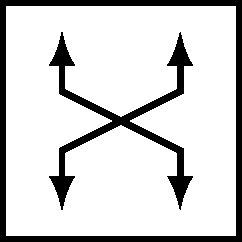
\includegraphics[width=0.9cm]{../common/fig-switch.pdf}
}
\providecommand{\router}{%
    
\includegraphics[width=0.9cm]{../common/fig-router.pdf}
}

% FIXME: scenario where 10.0.2.9 is machine A, then machine B
% FIXME: scenario where machine A and B both think they are 10.0.2.9
\begin{frame}[fragile]{}
\begin{tikzpicture}
\tikzset{
    computer/.style={inner sep=0mm,outer sep=0mm,execute at begin node={\computer}},
    computer alt/.style={inner sep=0mm,outer sep=0mm,execute at begin node={\computerAlt}},
    switch/.style={inner sep=0mm,outer sep=0mm,execute at begin node={\switch}},
    router/.style={inner sep=-1mm,outer sep=0mm,execute at begin node={\router},circle},
    connect/.style={draw,very thick,Latex-Latex},
    connect big/.style={draw,ultra thick,Latex-Latex},
    addr label/.style={align=left,font=\fontsize{9}{10}\selectfont\tt},
    arp table/.style={
        tight matrix,
        nodes={minimum height=.6cm},
        column 1/.style={nodes={text width=2.05cm,font=\small\tt}},
        column 2/.style={nodes={text width=1.75cm,font=\small\tt}},
        %row 1/.style={nodes={font=\small}},
    },
}
\begin{scope}[name prefix=first-]
    \node[computer,label={[addr label]north:MAC 77:\ldots:BB\\IP 10.0.2.2}] (n1-from) at (0, 0) {};
    \node[computer alt,label={[addr label]south:MAC 99:\ldots:BA\\IP 10.0.2.9}] (n1-to) at (0, -4) {};
    \node[switch] (sw) at (0, -2) {};
    \draw[connect] (n1-from) -- (sw);
    \draw[connect] (n1-to) -- (sw);
    \matrix[arp table,label={[label distance=0mm]north:.2's ARP table},inner sep=0mm,fill=white] 
        (arp table) at (2.75, -0.5) {
        10.0.2.9 \& 99:\ldots:BA \\
    };
\end{scope}
\begin{visibleenv}<2->
\draw[line width=2mm,black!50,dashed] (5.3, 2) -- ++(0, -8);
\begin{scope}[name prefix=second-,xshift=7cm]
    \node[computer,label={[addr label]north:MAC 77:\ldots:BB\\IP 10.0.2.2}] (n1-from) at (0, 0) {};
    \node[computer,label={[addr label]south:MAC \myemph<2>{CC:\ldots:01}\\IP 10.0.2.9}] (n1-to) at (2, -4) {};
    \node[switch] (sw) at (0, -2) {};
    \draw[connect] (n1-from) -- (sw);
    \draw[connect] (n1-to) -- (sw);
    \matrix[arp table,label={[label distance=0mm]north:.2's ARP table},inner sep=0mm,fill=white] 
        (arp table) at (2.75, -0.5) {
        10.0.2.9 \& |[alias=wrong mac box,alt=<2>{fill=red!10}]| 99:\ldots:BA \\
    };
    \begin{visibleenv}<2>
        \node[anchor=north,draw=red,very thick,align=left] at ([yshift=-.1cm]wrong mac box.south) {
            old entry prevents 10.0.2.2 \\
            from contacting new machine
        };
    \end{visibleenv}
\end{scope}
\node[anchor=south] at (2, 2) {Monday};
\node[anchor=south] at (8, 2) {Tuesday};
\end{visibleenv}
\end{tikzpicture}
\end{frame}

\begin{frame}{gratituous ARP requests}
    \begin{itemize}
    \item solution: send \textit{unsolicited} ARP messages
    \vspace{.5cm}
    \item CC:\ldots:01$\rightarrow$FF:\ldots:FF: request: who has 10.0.2.9, tell 10.0.2.9=CC:\ldots:01 
    \vspace{.5cm}
    \item<2-> request not reply b/c concerns about old/broken implementations
        \begin{itemize}
        \item ICMPv6 ND fixes this: \\
            message is `advertisement' ($\sim$ reply), not `solicitation' ($\sim$ request)
        \end{itemize}
    \end{itemize}
\end{frame}

\begin{frame}[fragile]{}
\begin{tikzpicture}
\tikzset{
    computer/.style={inner sep=0mm,outer sep=0mm,execute at begin node={\computer}},
    computer alt/.style={inner sep=0mm,outer sep=0mm,execute at begin node={\computerAlt}},
    switch/.style={inner sep=0mm,outer sep=0mm,execute at begin node={\switch}},
    router/.style={inner sep=-1mm,outer sep=0mm,execute at begin node={\router},circle},
    connect/.style={draw,very thick,Latex-Latex},
    connect big/.style={draw,ultra thick,Latex-Latex},
    addr label/.style={align=left,font=\fontsize{9}{10}\selectfont\tt},
    arp table/.style={
        tight matrix,
        nodes={minimum height=.6cm},
        column 1/.style={nodes={text width=2.05cm,font=\small\tt}},
        column 2/.style={nodes={text width=1.75cm,font=\small\tt}},
        %row 1/.style={nodes={font=\small}},
    },
}
\begin{scope}
    \node[computer,label={[addr label]north:MAC 77:\ldots:BB\\IP 10.0.2.2}] (n1-from) at (0, 0) {};
    \node[computer alt,label={[addr label]south:MAC 99:\ldots:BA\\IP \myemph<2>{10.0.2.9}}] (n1-toA) at (-2, -4) {};
    \node[computer alt,label={[addr label]south:MAC 09:\ldots:FE\\IP \myemph<2>{10.0.2.9}}] (n1-toB) at (2, -4) {};
    \node[switch] (sw) at (0, -2) {};
    \draw[connect] (n1-from) -- (sw);
    \draw[connect] (n1-toA) -- (sw);
    \draw[connect] (n1-toB) -- (sw);
\end{scope}
\end{tikzpicture}
\end{frame}

\begin{frame}{duplicate addresses}
    \begin{itemize}
    \item recommendations in RFC 5227 {\small ``IPv4 Address Conflict Detection''}
    \vspace{.5cm}
    \item probe for IP address before using it
        \begin{itemize}
        \item make sure to broadcast when starting to use address
        \item probably give up on address if conflict found
        \end{itemize}
    \item watch out for ARP messages indicating address in use
    \item on detecting conflict choose between:
        \begin{itemize}
        \item `defend' address with more gratituous requests
        \item give up address
        \end{itemize}
    \end{itemize}
\end{frame}


\subsection{ARP hijacking}

\usetikzlibrary{arrows.meta,calc,fit,matrix,shapes}
\providecommand{\computer}{%
    
\includegraphics[width=1cm]{../common/Noun_project_216.pdf}
}
\providecommand{\computerAlt}{%
    
\includegraphics[width=1cm]{../common/Noun_project_alt_cpu.pdf}
}
\providecommand{\switch}{%
    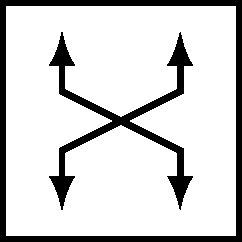
\includegraphics[width=0.9cm]{../common/fig-switch.pdf}
}
\providecommand{\router}{%
    
\includegraphics[width=0.9cm]{../common/fig-router.pdf}
}

\begin{frame}{ARP hijacking}
\begin{tikzpicture}
\tikzset{
    computer/.style={inner sep=0mm,outer sep=0mm,execute at begin node={\computer}},
    computer alt/.style={inner sep=0mm,outer sep=0mm,execute at begin node={\computerAlt}},
    switch/.style={inner sep=0mm,outer sep=0mm,execute at begin node={\switch}},
    router/.style={inner sep=-1mm,outer sep=0mm,execute at begin node={\router},circle},
    connect/.style={draw,very thick,Latex-Latex},
    connect big/.style={draw,ultra thick,Latex-Latex},
    addr label/.style={align=left,font=\fontsize{9}{10}\selectfont\tt},
    arp table/.style={
        tight matrix,
        nodes={minimum height=.6cm},
        column 1/.style={nodes={text width=2.05cm,font=\small\tt}},
        column 2/.style={nodes={text width=1.75cm,font=\small\tt}},
        %row 1/.style={nodes={font=\small}},
    },
    packet/.style={
        draw=blue,very thick,font=\tt\small,
        align=left,
    },
}
\begin{scope}
    \node[computer,label={[addr label]north:MAC 77:\ldots:BB\\IP 10.0.2.2}] (n1-from) at (0, 0) {};
    \node[computer alt,label={[addr label]south:MAC A5:\ldots:BA\\IP 10.0.2.9}] (n1-toA) at (-3, -4) {};
    \node[computer alt,label={[addr label]south:MAC 09:\ldots:FE},font=\Huge] (n1-toB) at (3, -4) {};
    \node[font=\huge] at (n1-toB) {\emoji{smiling-face-with-horns}};
    \node[switch] (sw) at (0, -2) {};
    \draw[connect] (n1-from) -- (sw);
    \draw[connect] (n1-toA) -- (sw);
    \draw[connect] (n1-toB) -- (sw);

    \begin{visibleenv}<2>
    \node[packet,anchor=north west] (blue spoof) at (3, 0) {
        09:\ldots:FE$\rightarrow$77:\ldots:BB \\
        10.0.2.9{\normalfont{} is }09:\ldots:FE
    };
    \node[packet,draw=violet,anchor=north west] (violet spoof) at (-1, -5) {
        09:\ldots:FE$\rightarrow$A5:\ldots:BA \\
        10.0.2.2{\normalfont{} is }09:\ldots:FE
    };
    \draw[blue,line width=1mm,dotted,-Latex] ([yshift=3mm]n1-toB.west) -- ([xshift=1mm]sw.center) -- (n1-from)
        coordinate[midway] (blue spoof point);
    \draw[violet,line width=1mm,dotted,-Latex] ([yshift=1mm]n1-toB.west) --
        ([xshift=-1mm,yshift=-1mm]sw.center) coordinate[midway] (violet spoof point) -- (n1-toA);
    \draw[blue,very thick] (blue spoof) -- (blue spoof point);
    \draw[violet,very thick] (violet spoof) -- (violet spoof point);
    \end{visibleenv}
    \begin{visibleenv}<3>
    \draw[Latex-Latex,red,line width=1mm] ([xshift=1mm]n1-from.south) -- ([xshift=1mm]sw.center)
        -- ([yshift=5mm]n1-toB.west);
    \draw[Latex-Latex,red,line width=1mm] ([yshift=-2mm]n1-toA.north east) -- ([yshift=-2mm]sw.center)
        -- ([yshift=0mm]n1-toB.west);
    \node[align=left,anchor=north west,draw=red,ultra thick] at (2, 0) {
        10.0.2.2 and 10.0.2.9 have \\
        ``poisoned'' ARP tables \\
        makes them send everything to attacker \\
        (instead of each other)
    };
    \end{visibleenv}
    % FIXME: ARP message to 10.0.2.2 with false 10.0.2.9
    % FIXME: ARP message to 10.0.2.9 with false 10.0.2.2
\end{scope}
\end{tikzpicture}
\end{frame}


% FIXME: ARP proxies?

\section{DHCP}
% FIXME: diagram with multiple DHCP servers
\usetikzlibrary{matrix}
\begin{frame}{autoconfiguration}
    \begin{itemize}
    \item how do hosts get address + default routing table?
    \item one answer: set manually
    \end{itemize}
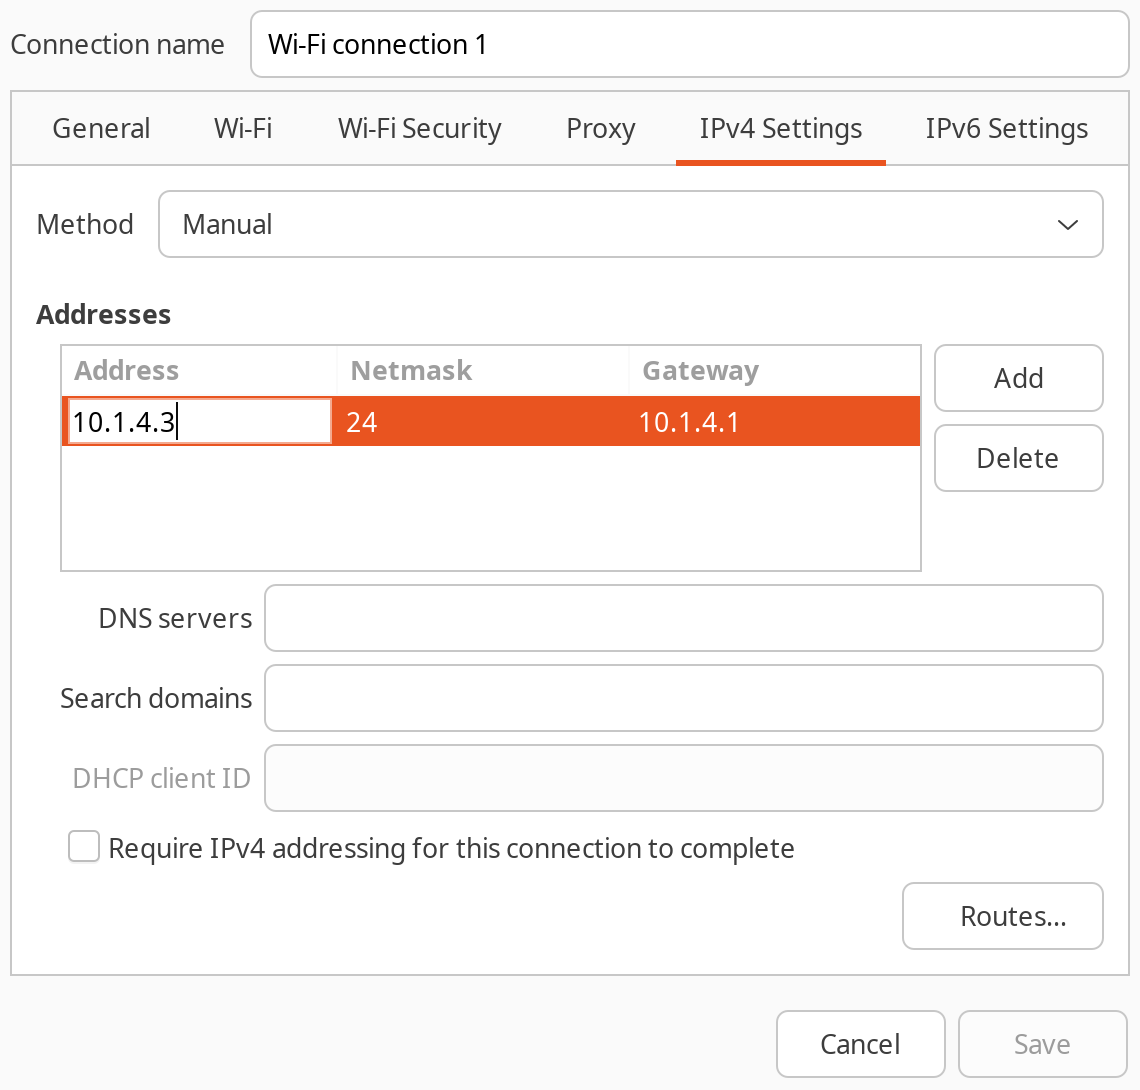
\includegraphics[width=0.5\textwidth]{../arp/ip-config-dialog}
\end{frame}

\begin{frame}{simple network config}
\begin{itemize}
    \item IP address: 10.0.2.45
    \item (sub)net mask: /25 (aka 255.255.255.128)
        \begin{itemize}
        \item varies which format is input
        \end{itemize}
    \item (default) gateway: 10.0.2.102
\end{itemize}
\begin{visibleenv}<2->
\begin{tikzpicture}
\matrix[tight matrix,
    nodes={minimum height=0.4cm},
    column 1/.style={nodes={text width=4cm}},
    column 2/.style={nodes={text width=3cm}},
    column 3/.style={nodes={text width=2cm}},
] {
addresses \& next hop \& device \\
10.2.0.0/25 \& (direct) \& out \\
default \& 10.2.0.102 \& out \\
};
\end{tikzpicture}
\end{visibleenv}
\end{frame}

\begin{frame}{DHCP messages (1)}
    \begin{itemize}
    \item protocol looks weird in packet traces because of history
    \item built on top of UDP + IP
    \item built as extension to older BOOTP (bootstrap protocol)
    \vspace{.5cm}
    \item common message format for different ``operations''
    \end{itemize}
\end{frame}

\begin{frame}{DHCP messages (2)}
    \begin{itemize}
    \item from client (looking to configure itself):
        \begin{itemize}
        \item DISCOVER (look for configuration server)
        \item REQUEST (get configuration from server)
        \end{itemize}
    \item from server (offering configurations):
        \begin{itemize}
        \item OFFER (`I am a configuration server')
        \item ACK (here's a configuration)
        \end{itemize}
    \end{itemize}
\end{frame}

\begin{frame}[fragile]{DHCP request example}
\begin{tikzpicture}
\tikzset{
    explain box/.style={draw=red,ultra thick,fill=white,align=left},
    hi box/.style={draw=red,line width=1mm},
}
\node[inner sep=0mm,anchor=north west] at (0, 0) {%
    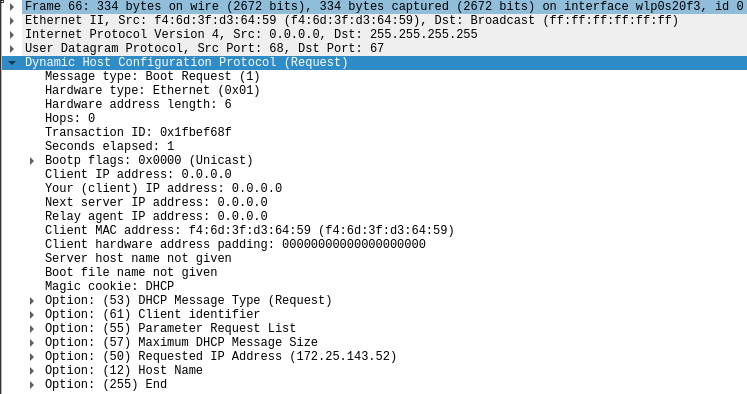
\includegraphics[width=\textwidth]{../arp/dhcp-request-wireshark.png}%
};
%\path[overlay,draw,help lines] (0, 0) grid (15, -8);
\begin{visibleenv}<2>
    \path[hi box] (0.4, -0.2) rectangle (13.2, -1.25);
    \node[anchor=north,explain box] at (7, -1.5) {
        built on IP+UDP rather than special protocol like ARP \\
        ~ \\
        sending to broadcast ethernet/IP address (all 1 bits)\\
        placeholder source IP of 0.0.0.0
    };
\end{visibleenv}
\begin{visibleenv}<3>
    \path[hi box] (0.5, -1.3) rectangle (5.2, -1.7);
    \node[anchor=north,explain box] at (8, -1.8) {
       `boot' probably because derived \\ from bootstrap protocol (BOOTP)
    };
\end{visibleenv}
\begin{visibleenv}<4>
    \path[hi box] (0.5, -3.2) rectangle (8.8, -4.6);
    \node[anchor=north,explain box] at (7, -5) {
        message format same in both directions, so \\
        fields here intended for use in response
    };
\end{visibleenv}
\end{tikzpicture}
\end{frame}

\begin{frame}{DHCP ACK example}
\begin{tikzpicture}
\tikzset{
    explain box/.style={draw=red,ultra thick,fill=white,align=left},
    hi box/.style={draw=red,line width=1mm},
}
\node[anchor=north west,inner sep=0mm] at (0, 0) {%
    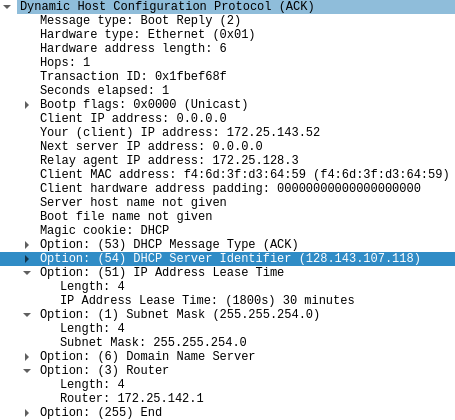
\includegraphics[width=0.55\textwidth]{../arp/dhcp-response3-wireshark.png}
};
%\path[overlay,draw,help lines] (0, 0) grid (15, -8);
\begin{visibleenv}<2>
    \draw[hi box] (0.6, -2.1) rectangle (5.7, -2.45);
    \draw[hi box] (0.6, -2.6) rectangle (5.5, -3.0);
    \draw[hi box] (0.4, -4.1) rectangle (7.5, -7.5);
    \node[explain box,anchor=north east] at (15, -2) {
        response (ACK) has address fields filled in
    };
\end{visibleenv}
\begin{visibleenv}<3>
    \draw[hi box] (0.6, -2.1) rectangle (5.7, -2.45);
    \draw[hi box] (0.4, -4.1) rectangle (7.5, -7.5);
    \matrix[fill=white,nodes={minimum height=0.4cm},
        column 1/.style={nodes={text width=4cm}},
        column 2/.style={nodes={text width=3cm}},
    ] (route table) at (15, -2) {
    addresses \& next hop \\
    172.25.142.0/23 \& (direct) \\
    default \& 172.25.142.1 \\
    };
    \node[anchor=north,explain box] at ([yshift=-.3cm]route table.north) {
        /23 = 255.255.254.0 mask \\
        ~ \\ 
        172.25.142.0 = \\
        172.25.143.52 bitwise-AND 255.255.254.0
    };
\end{visibleenv}
\end{tikzpicture}
\end{frame}

\begin{frame}{DHCP leases}
    \begin{itemize}
    \item DHCP ACKs specify a time limit
        \begin{itemize}
        \item (example from prior slide (UVa eduroam): 30 minutes)
        \end{itemize}
    \item need to be renewed (new REQUEST + ACK)
        \begin{itemize}
        \item REQUESTs can contain `desired address' (= current address when renewing)
        \end{itemize}
    \end{itemize}
\end{frame}
 % FIXME: incomplete


\subsection{DHCP relays}

\begin{frame}{how many DHCP servers?}
    \begin{itemize}
    \item DHCP assumption: broadcast to local network and there's the server
    \vspace{.5cm}
    \item conflicting goals:
        \begin{itemize}
        \item want broadcasts not to go to many machines (good performance)
        \item want to have few DHCP servers
        \end{itemize}
    \end{itemize}
\end{frame}

\begin{frame}{DHCP relays}
    % FIXME: picture from textbook
\end{frame}
 % FIXME: DHCP relay diagram

\subsection{DHCPv6}

% FIXME
% FIXME

\section{IPv6 autoconfiguration}

\begin{frame}{IPv6 autoconfiguration}
    \begin{itemize}
    \item in IPv4, autoconfiguration ``bolted on''
        \begin{itemize}
        \item one protocol to be assigned address (DHCP)
        \item one protoocl to communicate IP address to other nodes on network (ARP)
        \end{itemize}
    \item IPv6 was designed later, so they thought about it early
    \end{itemize}
\end{frame}

\begin{frame}{big network address assignment}
    \begin{itemize}
    \item IPv6 local networks are typically /64s
        \begin{itemize}
        \item $2^{64}$ address available for local network
        \end{itemize}
    \item why so big? allow easy address assignment
    \item StateLess Address Auto Configuration (SLAAC)
    \end{itemize}
\end{frame}

\begin{frame}{MAC-address based address assignment}
    \begin{itemize}
    \item let's say my local network is 2001:db8:4999:3333::/64
    \end{itemize}
{\fontsize{12}{13}\selectfont
\begin{tabular}{ll}
MAC address & IPv6 address \\
\tt \myemph<2>{11:22:33:44:55:66} & \tt 2001:db8:4999:3333:\myemph<2>{1122:33}ff:fe\myemph<2>{44:5566} \\
\tt \myemph<2>{01:A0:B3:CC:DD:FF} & \tt 2001:db8:4999:3333:\myemph<2>{01a0:b3}ff:fe\myemph<2>{cc:ddff} \\
\ldots & \ldots \\
\end{tabular}}
\end{frame}

\begin{frame}[fragile]{}
\begin{Verbatim}[fontsize=\fontsize{9}{10}\selectfont]
Network Working Group                                          T. Narten
Request for Comments: 3041                                           IBM
Category: Standards Track                                      R. Draves
                                                      Microsoft Research
                                                                                                                  January 2001
                                                                                                                     Privacy Extensions for Stateless Address Autoconfiguration in IPv6

...
Abstract

                                  ........  Use of the extension causes
   nodes to generate global-scope addresses from interface identifiers
   that change over time, even in cases where the interface contains an
   embedded IEEE identifier.  Changing the interface identifier (and the
   global-scope addresses generated from it) over time makes it more
   difficult for eavesdroppers and other information collectors to
   identify when different addresses used in different transactions
   actually correspond to the same node.
\end{Verbatim}
\end{frame}

\begin{frame}{late timeline}
\begin{itemize}
\item privacy extensions weren't default until
    \begin{itemize}
    \item MacOS X 10.7 (2011)
    \item Windows Vista (2007)
    \item Ubuntu 12.04 (2012)
    \end{itemize}
\end{itemize}
\end{frame}

% FIXME: wireshark example
\begin{frame}{SLAAC}
\begin{itemize}
\item uses ICMPv6 (same as for neighbor discovery)
\item two modes:
    \begin{itemize}
    \item when there's a router (get \textit{global} addresses)
    \item when there's only a local network (get \textit{link-local} addresses)
    \end{itemize}
\end{itemize}
\end{frame}

\begin{frame}{router adverisements}
\begin{itemize}
\item nodes send a ICMPv6 \textit{Router Solicitation} message
\item receive back a ICMPv6 \textit{Router Advertisement} which can have:
\vspace{.5cm}
\item \myemph<2>{prefix information}
    \begin{itemize}
    \item nodes choose address starting with prefix
    \item check for duplicates using neighbor discovery
    \end{itemize}
\item \myemph<3>{DNS information}
\item \myemph<4>{``managed configuration'' flag}
    \begin{itemize}
    \item nodes use DHCPv6 to get configuration
    \end{itemize}
\item \myemph<5>{``other configuration'' flag}
    \begin{itemize}
    \item nodes choose address using prefix, but more info avail via DHCPv6
    \end{itemize}
\end{itemize}
\end{frame}

% FIXME


\section{backup slides}
\begin{frame}{backup slides}
\end{frame}

\section{switched networks}

\usetikzlibrary{arrows.meta,calc,shapes}
\providecommand{\computer}{%
    
\includegraphics[width=1cm]{../common/Noun_project_216.pdf}
}
\providecommand{\switch}{%
    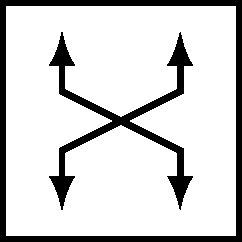
\includegraphics[width=0.9cm]{../common/fig-switch.pdf}
}
\providecommand{\router}{%
    
\includegraphics[width=0.9cm]{../common/fig-router.pdf}
}

\begin{frame}{recall: multi-access media}
\begin{tikzpicture}
\tikzset{
    connect/.style={draw,very thick,arrows={Latex-Circle[width=0.3cm,length=0.3cm]},
        alt=<2>{arrows={Latex-Circle[width=0.3cm,length=0.3cm,red]}}},
    computer/.style={inner sep=0mm,outer sep=0mm,execute at begin node={\computer}},
}
\draw[line width=1mm] (-5,-1.5) coordinate (wire start) -- (5, 1.5) coordinate (wire end);
\foreach \x/\d in {0/5cm,45/4cm,90/3cm,135/4cm,180/5cm,225/4cm,270/3cm,315/4cm} {
    \node[computer] (c-\x) at (\x:\d) {};
    \coordinate (connect-\x) at ($(wire start)!(c-\x.center)!(wire end)$);
    \draw[connect] (c-\x) -- (connect-\x) -- ([turn]0:.1cm);
}
\begin{visibleenv}<2-3>
\node[anchor=north west,fill=white,draw=black,thick,label={[font=\tiny]south:Ali at gwc.org.uk / Alistair1978 via Wikimedia commons / CC-BY-SA 2.5}] 
    (thicknet) at (4, 3.5) {
    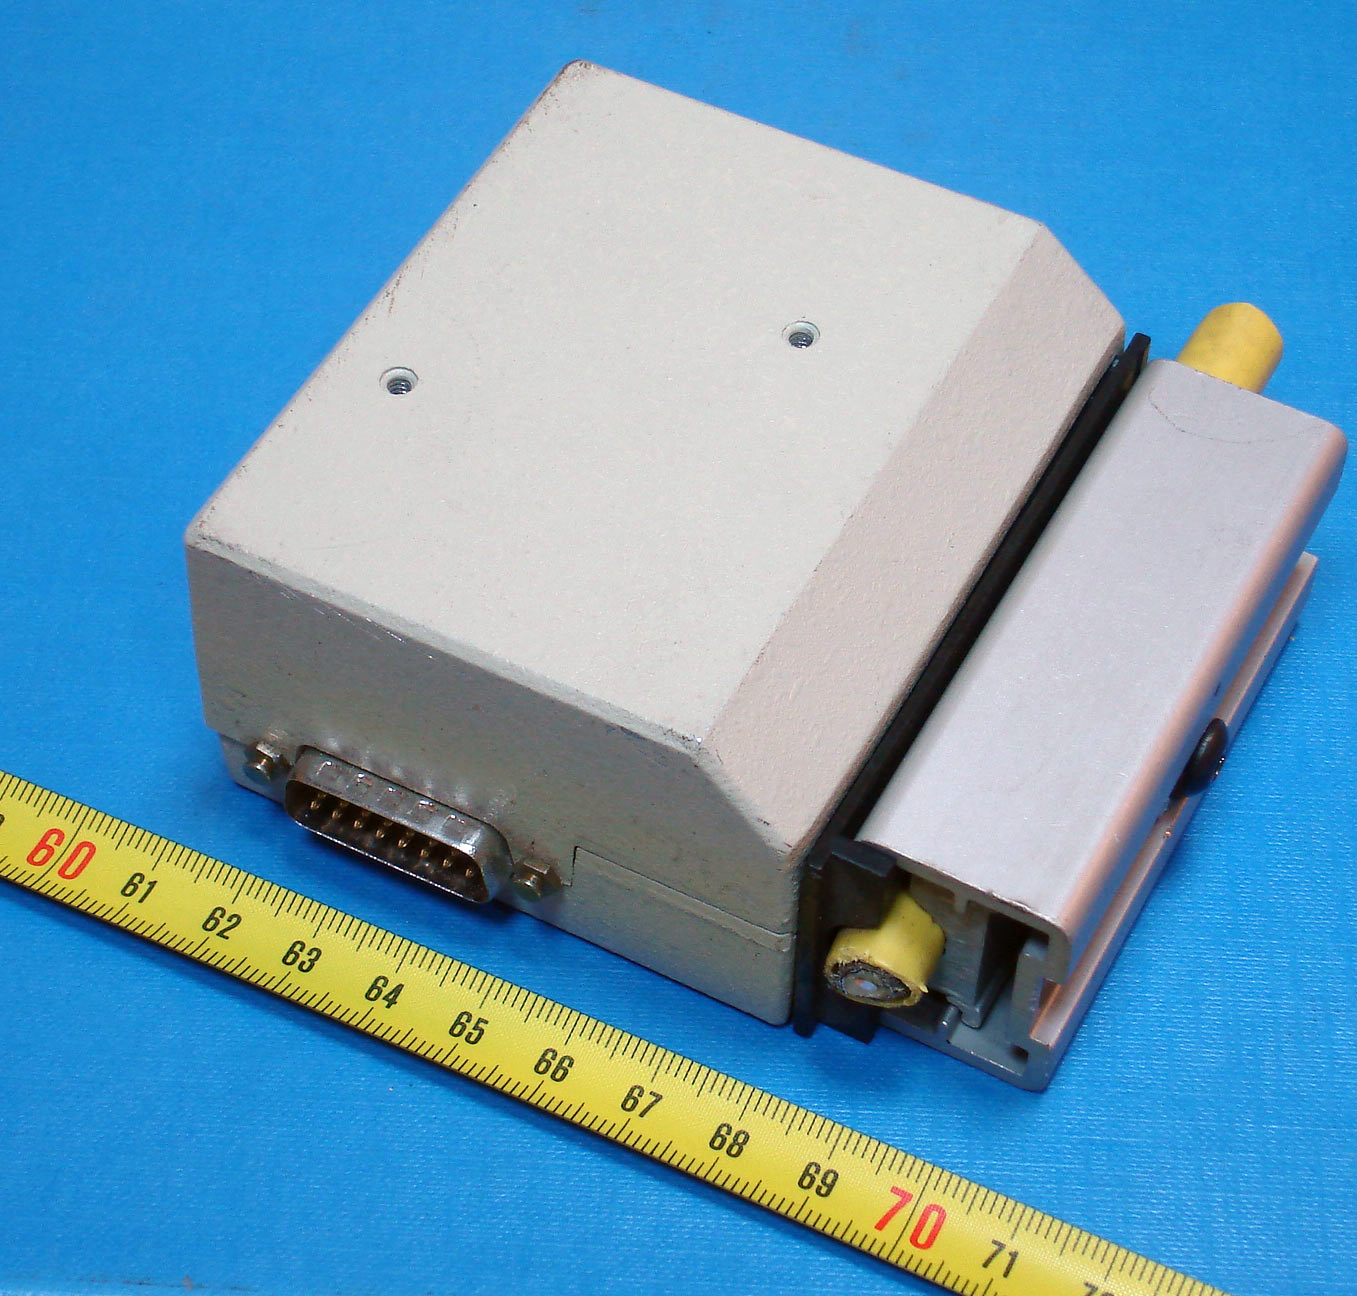
\includegraphics[width=4cm]{../intro/ThicknetTransceiver.jpeg}
};
\end{visibleenv}
\begin{visibleenv}<3>
\node[fill=white,draw=black,thick,anchor=north west] at ([yshift=-0.75cm]thicknet.south west) {
    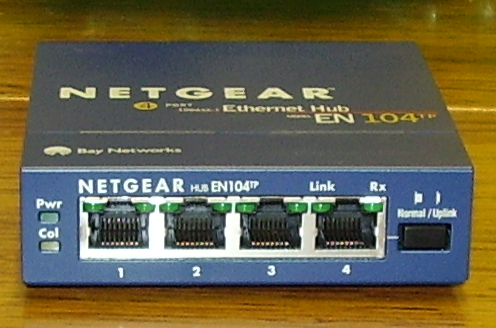
\includegraphics[width=4cm]{../intro/4_port_netgear_ethernet_hub}
};
% FIXME: also fiber splitter
\end{visibleenv}
\end{tikzpicture}
\end{frame}

\begin{frame}{recall: switched network}
\begin{tikzpicture}
\tikzset{
    computer/.style={inner sep=0mm,outer sep=0mm,execute at begin node={\computer}},
    switch/.style={inner sep=0mm,outer sep=0mm,execute at begin node={\switch},
                   alt=<1>{
                       fill=red!10,
                        label={[font=\small,label distance=0mm,text=red]south:`switch'}
                   }},
    connect/.style={draw,very thick,Latex-Latex,alt=<4>{red}},
    connect big/.style={draw,ultra thick,Latex-Latex,alt=<4>{red}},
}
\node[
      cloud,draw,opacity=0.25,very thick,aspect=2,
      minimum width=7cm,minimum height=4cm,
     ] (net-cloud) at (0,0) {};
\foreach \x/\d in {0/5cm,45/4cm,90/3cm,135/4cm,180/5cm,225/4cm,270/3cm,315/4cm} {
    \node[computer] (c-\x) at (\x:\d) {};
}
\node[switch] (s1) at (2,-0.5) {};
\node[switch] (s2) at (-1,0.5) {};
\node[switch] (s3) at (0,-1) {};
\draw[connect] (c-0) -- (s1);
\draw[connect] (c-45) -- (s1);
\draw[connect] (c-315) -- (s1);
\draw[connect] (c-90) -- (s2);
\draw[connect] (c-135) -- (s2);
\draw[connect] (c-180) -- (s2);
\draw[connect] (c-225) -- (s3);
\draw[connect] (c-270) -- (s3);
\draw[connect big] (s1) -- (s2);
\draw[connect big] (s1) -- (s3);
\coordinate (box loc) at (4cm, 4.5cm);
\end{tikzpicture}
\end{frame}

\begin{frame}{hubs and switches}
\begin{tikzpicture}
\node[fill=white,draw=black,thick,label={north:Hub}] (hub) {
    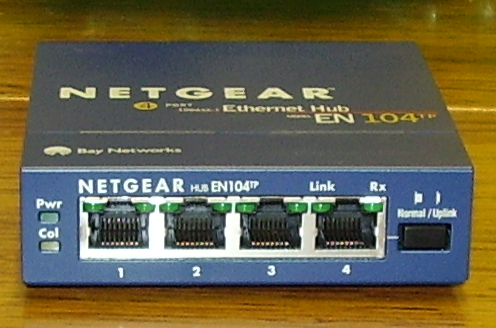
\includegraphics[width=6cm]{../intro/4_port_netgear_ethernet_hub}
};
\node[fill=white,draw=black,thick,anchor=north east,label={north:Switch}] (switch)  at (hub.north west){
    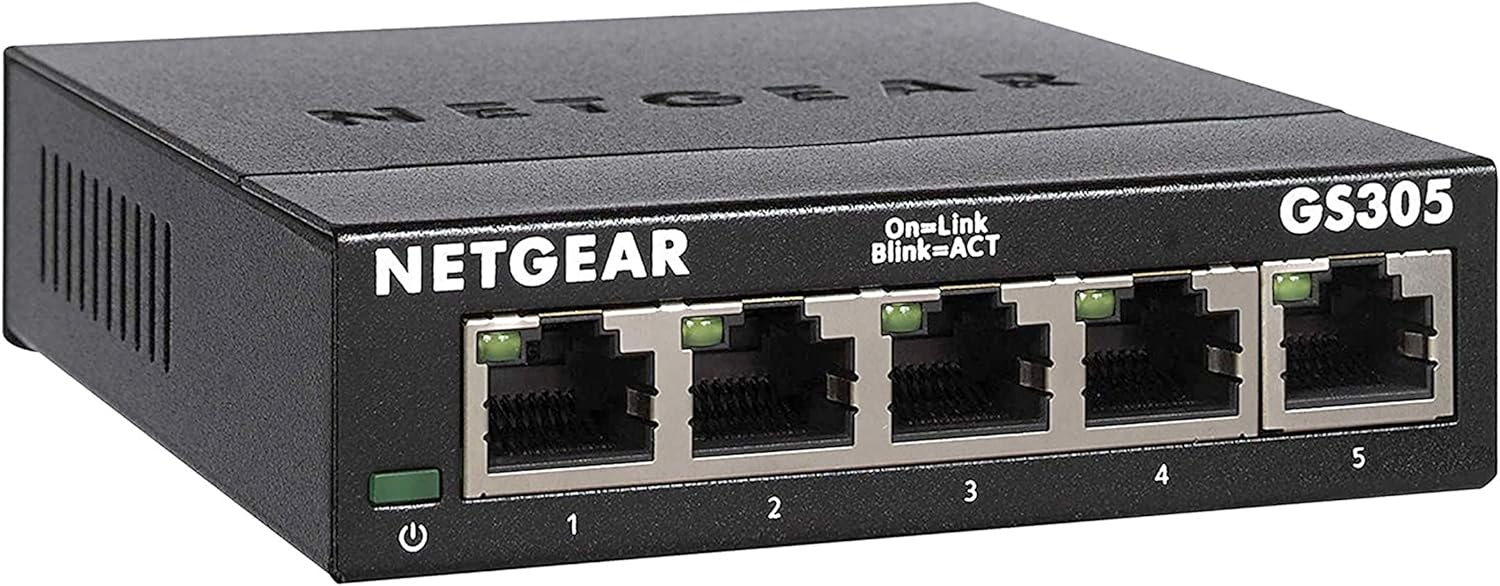
\includegraphics[width=6cm]{../switches/ModernNetgearSwitch}
};
\end{tikzpicture}
\begin{itemize}
\item difference is hidden inside
\item hub: electrically connects hosts --- as if shared wires
\item switch: decides what to send on each output
\end{itemize}
\end{frame}

\begin{frame}{history: multi-access to switched}
    \begin{itemize}
    \item a lot of early networking technology was multi-access
    \item wireless (wifi, cellular) and most home broadband still is
    \vspace{.5cm}
    \item most wired networks are \textit{switched}
        \begin{itemize}
        \item frames mostly directed to correct machine
        \end{itemize}
    \end{itemize}
\end{frame}

\begin{frame}{switching versus routing}
    \begin{itemize}
    \item switches --- forward frames for common network
    \item routers --- forward packets between networks
    \vspace{.5cm}
    \item basically same functionality
    \item differences:
        \begin{itemize}
        \item extra layer for internetwork packets
        \item different mechanism to decide where to forward
        \item switch forwarding typically simpler
        \end{itemize}
    \item will start with simpler switching
    \end{itemize}
\end{frame}



\section{datagrams and Ethernet format}

\usetikzlibrary{patterns}

\begin{frame}{typically sent on Ethernet}
\begin{tikzpicture}
\tikzset{
    box/.style={draw,thick},
    label/.style={font=\small},
    label large/.style={},
    missing/.style={pattern=north west lines},
    start and end/.style={alt=<2>{fill=red!10,text=red}},
    type field/.style={alt=<3-4>{fill=red!10,text=red}},
    destination address/.style={alt=<5-6>{fill=red!10,text=red}},
    source address/.style={alt=<7>{fill=red!10,text=red}},
}
\draw[start and end,box] (4, 0) rectangle (12, -1)
    node[midway,label] {preamble + start marker};
\draw[source address,box] (0, -1) rectangle (6, -2)
    node[midway,label] {source MAC address};
\draw[destination address,box] (6, -1) rectangle (12, -2)
    node[midway,label] {destination MAC address};
\draw[type field,box] (0, -2) rectangle (2, -3)
    node[midway,label] {type};
\draw[box] (2, -2) -- (12, -2) -- (12, -4) -- (0, -4) -- (0, -3) -| cycle;
    \node[label large] at (6, -3) {data (for next layer)};
\begin{visibleenv}<8>
\draw[red,ultra thick] (2, -2) -- (2, -3);
\draw[box,red,ultra thick,fill=white] (4.5, -3) rectangle (11.5, -4) 
    node[midway,label] {sometimes extra stuff (``tags'')};
\end{visibleenv}
\draw[box] (0, -4) rectangle (4, -5) node[midway,label] {checksum};
\draw[start and end,box,missing] (4, -4) rectangle (12, -5)
    node[midway,label,fill=white] {`interpacket gap'};
\draw[start and end,box,missing] (0, -5) rectangle (4, -6);
\begin{visibleenv}<2>
\node[align=left,draw=red,ultra thick,fill=white] at (6, -3) {
    explicit start marker \\
    end indicated by `gap' between signals
};
\end{visibleenv}
\begin{visibleenv}<3>
\node[align=left,draw=red,ultra thick,fill=white] at (8, -3) {
    type field indicates which next layer in use \\
    often varies on frame-by-frame basis \\
};
\end{visibleenv}
\begin{visibleenv}<4>
\node[align=left,draw=red,ultra thick,fill=white] at (8, -3) {
    actually \texttt{type/length} for historical reasons \\
    but most commonly used for type these days
};
\end{visibleenv}
\begin{visibleenv}<5>
\node[align=left,draw=red,ultra thick,fill=white] at (6, -4) {
    destination address indicates who frame is for \\
    present regardless of whether switching is in use \\
    ~ \\
    each host \myemph{filters} out frames for `wrong' destination address
};
\end{visibleenv}
\begin{visibleenv}<6>
\node[align=left,draw=red,ultra thick,fill=white] at (6, -4) {
    since destination address always present \\
    as last resort, switches can send every frame to everyone \\
    ~ \\
    will still work, just much less efficient
};
\end{visibleenv}
\begin{visibleenv}<7>
\node[align=left,draw=red,ultra thick,fill=white] at (6, -4) {
    who the frame came from \\
    gives `return address' for sending replies \\
    ~ \\
    will also be used by switches
};
\end{visibleenv}
\end{tikzpicture}
\end{frame}

\begin{frame}{MAC addresses}
    \begin{itemize}
    \item MAC [media access control] addresses
    \item used by Ethernet, Wifi, and lots of other protocols
    \item 48-bit number written in hex: \texttt{01:23:45:67:89:AB}
        \begin{itemize}
        \item (sometimes seperated with \texttt{-} instead of \texttt{:})
        \end{itemize}
    \item assigned by IEEE to networking manufacturers in blocks
        \begin{itemize}
        \item Institution of Electrical and Electronics Engineers
        \item example: \texttt{00:02:B3:}\ldots, \texttt{00:03:47:}\ldots, (and many more) for Intel
        \end{itemize}
    \vspace{.5cm}
    \item individual addresses hard-coded in networking hardware
        \begin{itemize}
        \item uniquely identify port/device
        \end{itemize}
    \end{itemize}
\end{frame}

\begin{frame}{special MAC addresses}
    \begin{itemize}
    \item \texttt{00:00:00:00:00:00} (all zeroes)
    \item \texttt{FF:FF:FF:FF:FF:FF} (all ones), \texttt{FF:}\ldots
        \begin{itemize}
        \item special destination meaning ``send to everyone'' (on this network)
        \item called \textit{broadcast}
        \end{itemize}
    \item \texttt{01:80:C2:}\ldots, \texttt{33:33:}\ldots, (and some more)
        \begin{itemize}
        \item special destinations representing multiple receivers
        \item example: `all IPv6 routers on this network' (\texttt{33:33:00:00:00:02})
        \item called \textit{multicast}
        \end{itemize}
    \end{itemize}
\end{frame}

\begin{frame}{larger MAC addresses}
    \begin{itemize}
    \item IEEE now calls MAC address EUI-48 (48-bit Extended Unique Identifier)
    \vspace{.5cm}
    \item also created EUI-64, with 64-bit addresses
        \begin{itemize}
        \item way of mapping EUI-48s to EUI-64s
        \item turns out 48 bits might have been low
        \end{itemize}
    \item I'm not sure what status is on switching to 64-bit addresses
        \begin{itemize}
        \item IEEE 802.15.4 (used in ZigBee, 6LoWPAN, some others) uses EUI-64
        \item I don't know other local network protocols that do
        \end{itemize}
    \end{itemize}
\end{frame}


% FIXME: example in wireshark

\subsection{versus virtual circuits}

\begin{frame}{datagram idea}
    \begin{itemize}
    \item can always send something to anyone on network
        \begin{itemize}
        \item just put destination MAC in frame
        \end{itemize}
    \item no need for reservations/`connections'/etc.
        \begin{itemize}
        \item not like the interface you've seen with [TCP] sockets
        \end{itemize}
    \vspace{.5cm}
    \item not the only model for networks (and internetworks)
    \end{itemize}
\end{frame}

\begin{frame}{virtual circuit}
    \begin{itemize}
    \item other model: virtual circuit
    \item two machines setup a `circuit'
        \begin{itemize}
        \item some sort of `special' messages to do this
        \end{itemize}
    \item switches/routers \myemph{reserve resources} for circuit
        \begin{itemize}
        \item ``gaurenteed'' bandwidth
        \end{itemize}
    \item transmitted data must be part of estabished circuit
    \vspace{.5cm}
    \item example: ATM (Asynchronous Transfer Mode)
        \begin{itemize}
        \item used (?historically?) by some telephone networks
        \end{itemize}
    \end{itemize}
\end{frame}

\end{document}
